\documentclass[a4paper,12pt]{article}

%%% Работа с русским языком

\usepackage{cmap}					% поиск в PDF
\usepackage{mathtext} 				% русские буквы в формулах
\usepackage[T2A]{fontenc}			% кодировка
\usepackage[utf8]{inputenc}			% кодировка исходного текста
\usepackage[english,russian]{babel}	% локализация и переносы
\usepackage{indentfirst}            % красная строка в первом абзаце
\usepackage[unicode]{hyperref}
\usepackage{epigraph}
\frenchspacing                      % равные пробелы между словами и предложениями

%%% Дополнительная работа с математикой
\usepackage{amsmath,amsfonts,amssymb,amsthm,mathtools} % пакеты AMS
\usepackage{bbm} % Blackboard bold для цифр
\usepackage{icomma}                                    % "Умная" запятая

\renewcommand{\phi}{\ensuremath{\varphi}}
\renewcommand{\kappa}{\ensuremath{\varkappa}}
\renewcommand{\le}{\ensuremath{\leqslant}}
\renewcommand{\leq}{\ensuremath{\leqslant}}
\renewcommand{\ge}{\ensuremath{\geqslant}}
\renewcommand{\geq}{\ensuremath{\geqslant}}
\renewcommand{\emptyset}{\ensuremath{\varnothing}}

\newcommand{\cl}{\text{cl }}
\newcommand{\setint}{\text{int }}

\theoremstyle{plain}
\newtheorem{theorem}{Теорема}[section]
\newtheorem{lemma}{Лемма}[section]
\newtheorem{proposition}{Утверждение}[section]
\newtheorem*{corollary}{Следствие}
\newtheorem*{exercise}{Упражнение}

\theoremstyle{definition}
\newtheorem{definition}{Определение}[section]
\newtheorem*{note}{Замечание}
\newtheorem*{reminder}{Напоминание}
\newtheorem*{example}{Пример}
\newtheorem*{tasks}{Вопросы и задачи}

\theoremstyle{remark}
\newtheorem*{solution}{Решение}

%%% Оформление страницы
\usepackage{extsizes}     % Возможность сделать 14-й шрифт
\usepackage{geometry}     % Простой способ задавать поля
\usepackage{setspace}     % Интерлиньяж
\usepackage{enumitem}     % Настройка окружений itemize и enumerate
\setlist{leftmargin=25pt} % Отступы в itemize и enumerate

\geometry{top=25mm}    % Поля сверху страницы
\geometry{bottom=30mm} % Поля снизу страницы
\geometry{left=20mm}   % Поля слева страницы
\geometry{right=20mm}  % Поля справа страницы

\begin{document}
\tableofcontents
\newpage

\section{Основные понятия, простейшие типы дифф. уравнений}
\subsection{Основные понятия}
\begin{definition}
	Уравнение вида
	\begin{equation}
		\label{SDE}
		F(x,\, y,\, \ldots,\, y^{(n)}) = 0
	\end{equation}

	называется обыкновенным дифференциальным уравнением $n$-го порядка.
\end{definition}

\begin{definition}
	Функция $\phi(x)$, определённая на $I$ вместе со своими $n$ производными, называется решением уравнения (\ref*{SDE}), если:

	\begin{enumerate}
		\item $\phi$ и все её $n$ производных непрерывны на $I$.
		\item $\forall x \in I:\: (x,\, \phi(x),\, \phi'(x),\, \ldots,\, \phi^{(n)}(x)) \in \Omega$, где $\Omega$ - область определения $F$.
		\item $\forall x \in I:\: F(x,\, \phi(x),\, \phi'(x),\,\ldots,\,\phi^{(n)}) = 0$
	\end{enumerate}
\end{definition}

\begin{definition}
	Решение $y = \phi(x),\, x \in \langle a,\, b\rangle$ уравнения (\ref*{SDE}) называется продолжаемым вправо, если существует такое решение $y = \psi(x),\, x \in \langle a,\, b_1 \rangle,\, \langle a,\, b\rangle \subset \langle a,\, b_1 \rangle$, что $\phi(x) \equiv \psi(x)$ при $x \in \langle a,\, b\rangle$

	Аналогично определяется продолжение решения влево.
\end{definition}

\begin{definition}
	Решение называется непродолжаемым, если его нельзя продолжить ни вправо, ни влево.
\end{definition}

\begin{definition}
	Система дифференциальных уравнений называется автономной, если она имеет вид:
	\[
		\frac{dx_k}{dt} = f_k(x_1,\, \ldots,\,x_n);\; k = 1,\,\ldots,\,n
	\]
	также очень часто автономные системы записываются в компактном векторном виде:
	\begin{equation}
		\label{Autonomius}
		\dot{x} = F(x),\, x \in \Omega \subseteq E^n
	\end{equation}

\end{definition}

\begin{definition}
	Непрерывно дифференцируемая в $\Omega$ функция $u(x)$ называется первым интегралом системы $(\ref*{Autonomius})$, если $\forall t \in T:\: u(x(t)) \equiv const$ для каждого решения $x(t)$ этой системы.
\end{definition}

\begin{definition}
	Если поставить в соответствие каждой точке $(x,\, y)$ некоторого множества $\Omega \subseteq E^2$ вектор с координатными представлением $(1,\, f(x,\,y))$, то полученное векторное множество принято называть полем направлений ОДУ первого порядка.
\end{definition}

\begin{definition}
	Векторное поле - это отображение, которое сопоставляет каждой точке некоторого пространства вектор
\end{definition}

\begin{definition}
	Пусть $x(t)$ есть частное решение системы (\ref*{Autonomius}), тогда вектор-функция $x(t),\, t \in T$, параметрически задаёт некоторую линию в $E^n$, называемую фазовой траекторией этой системы.
\end{definition}

\begin{definition}
	Совокупность фазовых траекторий для всех частных решений будем именовать фазовым портретом системы (\ref*{Autonomius})
\end{definition}

\begin{definition}
	График функции $y = \phi(x)$ можно рассматривать как геометрическое представление частного решения уравнения (\ref*{SDE}). Этот график обычно называют интегральной кривой уравнения (\ref*{SDE}).
\end{definition}

\subsection{Простейшие типы уравнений первого порядка}

\subsubsection*{Уравнения с разделяющимися переменными}
\begin{definition}
	Уравнения с разделяющимися переменными - это уравнения, которые могут быть записаны в виде

	\[y' = f(x)g(y)\; f(x) \in C(I_1),\, g(y) \in C(I_2)\]

	или же в виде

	\[M(x)N(y)dx + P(x)Q(y)dy = 0\]
\end{definition}

\begin{note}
	Если же $y_k \in C(I_2)$ решение уравнения $g(y) = 0$, то $y \equiv y_k$ -- решение дифф. уравнения
\end{note}

Если же $y(x)$ нигде не принимает значение $y_k$, то $g(y) \neq 0$, а потому мы можем делить на него. Значит, чтобы решить исходное уравнение, необходимо разделить переменные, то есть, привести уравнение к такой форме, чтобы при дифференциале $dx$ стояла функция, зависящая лишь от $x$, а при дифференциале $dy$ -- функция, зависящая от $y$.

\subsubsection*{Однородные уравнения}
\begin{definition}
	Функция двух переменных $f(x,\,y)$ называется однородной степени $m$, если для всех $t$ справедливо соотношение:
	\[f(tx,\,ty) = t^mf(x,\,y)\]
\end{definition}

\begin{definition}
	Однородным дифференциальным уравнением называется уравнение вида
	\[M(x,\,y)dx + N(x,\,y)dy = 0\]
	если $M(x,\,y)$ и $N(x,\,y)$ -- однородные функции одной и той же степени $m$.
\end{definition}

Однородное уравнение приводится к уравнению с разделяющимися переменными с помощью замены искомой функции $y(x)$ по формуле:
\[t(x) = \frac{y(x)}{x}\]

Тогда производная $y'$ и дифференциал $dy$ заменяются по формулам:
\[y' = t'x + t,\,\, dy = tdx + xdt\]

\subsubsection*{Линейные уравнения}
\begin{definition}
	Линейным уравнением первого порядка называется уравнение, линейное относительно искомой функции $y(x)$ и её производной, то есть, уравнения вида
	\[y' + a(x)y = b(x)\;\;\; a(x),\,b(x) \in C(I)\]

	Функция $b(x)$ называется свободным членом уравнения.

	Уравнение \[y' + a(x)y = 0\] называется линейным однородным уравнением, соответствующим изначальному линейному уравнению.
\end{definition}

Покажем, что однородное уравнение является уравнением с разделяющимися перменными

\[y' + a(x)y = 0 \Rightarrow \int \frac{dy}{y} = -\int a(x) dx \Rightarrow |y| = e^C \cdot e^{-\int_{x_0}^x a(t) dt}\]

Объединяя все решения, получаем общее решение:
\[y_0 = C \exp\left[-\int_{x_0}^x a(t) dt\right]\]

Будем искать частное решение исходного линейного уравнения методом вариации постоянной:
\[y_{\textbf{ч}} = C(x) \cdot \exp\left[-\int_{x_0}^x a(t) dt\right]\]

\subsubsection*{Уравнение Бернулли}
\begin{definition}
	Нелинейное уравнение первого порядка вида
	\[y' + a(x)y = b(x)y^m,\;\;\; m \neq 0,\, m \neq 1,\, a,\,b \in C(I)\]
	называется уравнением Бернулли.
\end{definition}

Заметим, что $y = 0$ -- решение уравнения Бернулли при $m > 0$.

Если $y \neq 0$, то, разделив уравнение на $y^m$ и вводя новую неизвестную функцию $z = y^{1 - m}$, относительно функции $z$ получаем линейное уравнение.

\subsubsection*{Уравнение Рикатти}
\begin{definition}
	Нелинейное уравнение первого порядка вида
	\[y' = a(x)y^2 + b(x)y + c(x) \;\;\; a,\,b\,\,c \in C(I)\]
	называется уравнением Рикатти
\end{definition}

В отличие от всех уравнений, рассматривавшихся ранее, уравнение Рикатти не всегда интегрируется в квадратурах. Чтобы решить его, необходимо знать хотя бы одно частное решение $y = y_1(x)$ этого уравнения. Тогда замена $y = y_1 + z$ приводит это уравнение к уравнению Бернулли.

\subsubsection*{Логистическое уравнение Ферхюльста}
\begin{note}
	Исходные предположения для вывода уравнения при рассмотрении популяционной динамики выглядит следующим образом:
	\begin{itemize}
		\item Скорость размножения популяции пропорциональна её текущей численности при прочих равных условиях
		\item Скорость размножения популяции пропорциональна количеству доступных ресурсов при прочих равных условиях.
	\end{itemize}
\end{note}

\begin{definition}
	Обозначая через $P$ численность популяции, а время - $t$, модель можно свести к дифференциальному уравнению
	\[\frac{dP}{dt} = rP(1 - \frac{P}{K})\]
	где параметр $r$ характеризует скорость роста, а $K$ -- максимальную возможную численность популяции.
\end{definition}

\begin{note}
	Точным решения является логистическая функция, S-образная кривая:
	\[P(t) = \frac{KP_0e^{rt}}{K + P_0(e^{rt}-1)}\] где $P_0$ -- начальная популяция, и $\lim\limits_{t \to \infty} P(t) = K$.
\end{note}

\subsection{Уравнения в полных дифференциалах, интегрирующий множитель}
\subsubsection*{Уравнения в полных дифференциалах}
\begin{definition}
	Это уравнение
	\[M(x,\,y)dx + N(x,\,y)dy = 0\]
	называется уравнением в полных дифференциалах, если его левая часть является дифференциалом некоторой гладкой функции $F(x,\,y)$. Тогда это уравнение можно переписать в виде $dF(x,\,y) = 0$, так что его решение будет иметь вид
	\[F(x,\,y) = C\]
\end{definition}

\begin{proposition}
	Если функции $M(x,\,y)$ и $N(x,\,y)$ определены и непрерывны в некоторой односвязной области $\Omega$ и имеют в ней непрерывные частные производные по $x$ и по $y$, то изначальное уравнение будет уравнением в полных дифференциалах тогда и только тогда, когда выполняется тождество
	\[\frac{\partial M(x,\,y)}{\partial y} \equiv \frac{\partial N(x,\,y)}{\partial x}\]
\end{proposition}

\subsubsection*{Интегрирующий множитель}
Пусть дано уравнение в дифференциалах, которое не является уравнением в полных дифференциалах.

\begin{definition}
	Функция $\mu(x,\,y) \neq 0$ называется интегрирующим множителем для исходного уравнения, если уравнение
	\[\mu(x,\,y)(M(x,\,y)dx + N(x,\,y)dy) = 0\]
	является уравнением в полных дифференциалах. Отсюда следует, что функция $\mu$ удовлетворяет условию
	\[\frac{\partial(\mu M)}{\partial y} \equiv \frac{\partial(\mu N)}{\partial x}\]
	Это равенство даёт уравнение в частных производных первого порядка для $\mu(x,\,y):$
	\[N\frac{\partial\mu}{\partial x} - M\frac{\partial\mu}{\partial y} = \left(\frac{\partial M}{\partial y} - \frac{\partial N}{\partial x}\right)\mu\]
	Поделив обе части последнего уравнения на $\mu$, перепишем его в виде:
	\[N\frac{\partial \ln\mu}{\partial x} - M\frac{\partial \ln\mu}{\partial y} = \frac{\partial M}{\partial y} - \frac{\partial N}{\partial x}\]
\end{definition}

\subsubsection*{Точные и замкнутые 1-формы, лемма Пуанкаре}
\begin{definition}
	Форма $\omega$ называется точной, если существует гладкая функция $F$, такая что $\omega = dF$
\end{definition}

\begin{definition}
	Форма $\omega = F_1dx_1 + \cdots + F_mdx_m$ называется замкнутой, если
	\[\forall k,\,i:\: \frac{\partial F_i}{\partial x_k} = \frac{\partial F_k}{\partial x_i}\]
\end{definition}

\begin{definition}
	Область $\Omega \subseteq \mathbb{R}^m$ называется звёздной, если для некоторой точки $p \in \Omega$ и для любой другой точки $q \in \Omega$ отрезок $[p,\, q]$ полностью содержится в $\Omega$.
\end{definition}

\begin{lemma}
	В звёздной области любая замкнутая $C^1$-гладкая дифференциальная 1-форма точна.
\end{lemma}

\begin{proof}
	Будем считать, что точка $p$ из определения звёздной области находится в начале координат. Пусть $\omega$ -- замкнутая форма, $\omega = A_1dx_1 + \ldots A_ndx_n$.

	Заметим, что для любой точки $x = (x_1,\,\ldots,\,x_n)$ и любой функции $G:\: \mathbb{R}^n \to \mathbb{R}$
	\[G(x) - G(0) = \int_{[0,\,x]}dG = \int_0^1\left(x_1\frac{\partial G}{\partial x_1}(tx) + \cdots + x_n\frac{\partial G}{\partial x_n}(tx)\right)dt\]
	мы параметризовали отрезок $[0,\,x] \subset \mathbb{R}^n$ параметром $t$. Пользуясь этим равенством, можно восстановить любую функцию по набору её производных.

	Поэтому естественно определить $F$ таким образом:
	\[F := \int_0^1 \sum_{i = 1}^n x_iA_i(xt)dt\]
	Нам осталось проверить, что $\frac{\partial F}{\partial x_s} = A_s$. Действительно,
	\begin{align*}
		\frac{\partial F}{\partial x_s} = \int_0^1 \frac{\partial}{\partial x_s} \sum_{i = 1}^n x_iA_i(xt)dt = \int_0^1 A_s(tx) + \sum_{i = 1}^n x_i \frac{\partial}{\partial x_s}A_i(tx)dt = \\
		= \int_0^1 A_s(tx) + \sum_{i = 1}^n x_i \frac{\partial}{\partial x_i}A_s(tx)dt = \int_0^1 \frac{d}{dt}(tA_s(tx))dt = A_s(x)
	\end{align*}
	Итак, $dF = A_1dx_1 + \cdots + A_ndx_n = \omega$.
\end{proof}

\subsubsection*{Гамильтоновые векторные поля на плоскости}
\begin{definition}
	Пусть $H:\: \mathbb{R}^2 \to \mathbb{R} \in C^1(\mathbb{R}^2)$. Тогда векторное поле
	$\vec{v}: \begin{cases}
			\dot{x} = -\frac{\partial H}{\partial y}(x,\,y) \\
			\dot{y} = \frac{\partial H}{\partial x}(x,\,y)
		\end{cases}$ называется гамильтоновым тогда и только тогда, когда $\text{div }\vec{v} = 0$
\end{definition}

\subsection{Методы понижения порядка для некоторых простейших типов дифференциальных уравнений. Уравнения первого порядка, не разрешённые относительно производной.}
\subsubsection*{Методы понижения порядка дифференциальных уравнений.}
\begin{enumerate}
	\item Пусть $F(x,\, y^{(k)},\,\ldots,\,y^{(n + k)}) = 0$

	      Замена: $z = y^{(k)}$, сводим к уравнению $F(x,\, z,\, z',\,\ldots,\,z^{(n)}) = 0$
	\item Пусть $F$ явно не зависит от $x$: $F(y,\, y',\,\ldots,\,y^{(n)}) = 0$

	      Замена: $y$ -- новая независимая переменная, $y' = p = p(y)$, то есть $y''_{xx} = p'_x = p'y'=p'p$
	\item Обобщённо-однородное уравнение

	      Пусть $\exists m,\,k:\: \forall \lambda > 0:\: F(\lambda x,\, \lambda^m y,\, \lambda^{m - 1}y',\,\ldots,\,\lambda^{m - n}y^{(n)}) = \lambda^k F(x,\,y,\,y',\,\ldots,\,y^{(n)})$

	      Замена: $x = e^t,\, y = z(t)e^{mt}$
	\item Однородные уравнения

	      Пусть $\exists k:\: \forall \lambda > 0:\: F(x,\, \lambda y,\, \lambda y',\,\ldots,\, \lambda y^{(n)}) = \lambda^k F(x,\,y,\,y',\,\ldots,\,y^{(n)})$

	      Замена: $y' = z(x)y,\, y'' = (z(x)y)' = z'y + zy' = z'y + z^2y = y(z + z^2)$
\end{enumerate}

\subsubsection*{Уравнения первого порядка, не разрешённые относительно производной}
\begin{definition}
	Уравнение первого порядка, не разрешённое относительно производной -- это уравнение вида
	\[F(x,\,y,\,y') = 0\]
	где $F(x,\,y,\,y')$ -- заданная непрерывная функция в некоторой непустой окрестности $G \subseteq \mathbb{R}^3_{(x,\,y,\,p)}$ с декартовыми прямоугольными координатами $x,\,y,\,p$.
\end{definition}

\begin{note}
	В общем случае для решения уравнения применяется метод введения параметра, который позволяет свести решение исходного уравнения к решению некоторого уравнения первого порядка в симметричной форме.

	Сам метод: положим $y' = p$ и рассмотрим систему
	\begin{equation}
		\label{BASE}
		\begin{cases}
			F(x,\,y,\,p) = 0 \\
			dy = pdx
		\end{cases}
	\end{equation}
\end{note}

\begin{proposition}
	Проектирование $\pi$ поверхности $F(x,\,y,\,p) = 0$ на плоскость $(x,\,y)$ вдоль оси $p$ переводит траектории поля в интегральные кривые системы (\ref*{BASE}).

	В тех точках поверхности, где производная $\frac{\partial F}{\partial p} \neq 0$, отображение $\pi$ является локальным диффеоморфизмом.
\end{proposition}

\begin{definition}
	Точки поверхности $F(x,\,y,\,p) = 0$, в которых производная $\frac{\partial F}{\partial p} = 0$, называются особыми точками уравнения (\ref*{BASE}).
\end{definition}

\begin{definition}
	Множество всех особых точек называется криминантой, а её проекция на плоскость $(x,\,y)$ -- дискриминантной кривой уравнения (\ref*{BASE}).
\end{definition}

\begin{definition}
	Решение уравнения (\ref*{BASE}) называется особым, если его интегральная кривая принадлежит дискриминантной кривой.
\end{definition}

\begin{note}
	Решение уравнения (\ref*{BASE}) можно трактовать, как траектории движения по этой поверхности, задаваемого векторным полем
	\begin{equation}
		\label{PODN_POLE}
		\begin{cases}
			\dot{x} = \frac{\partial F}{\partial p}  \\
			\dot{y} = p\frac{\partial F}{\partial p} \\
			\dot{p} = -\left(\frac{\partial F}{\partial x} + p\frac{\partial F}{\partial y} \right)
		\end{cases}
	\end{equation}
\end{note}

\begin{definition}
	Другой важной кривой является кривая перегибов, состоящая из всех точек поверхности $F(x,\,y,\,p) = 0$, в которых третья компонента поля (\ref*{PODN_POLE}) обращается в нуль.
\end{definition}

\begin{proposition}
	Криминанта и кривая перегибов связаны некоторым двойственным соотношением: преобразование Лежандра $(x,\,y,\,p) \to (p,\, xp - y,\, x)$ переводит всякую интегральную кривую $\gamma$ уравнения (\ref*{BASE}) в интегральную кривую $\gamma^*$ сопряжённого уравнения $F(p,\, xp - y,\, x) = 0$
\end{proposition}

\section{Задача Коши}
\subsection{Прицип сжимающих отображений}
\begin{definition}
	Точка $x^* \in X$ называется неподвижной точкой отображения $\Phi$, если $\Phi(x^*) = x^*$.
\end{definition}

\begin{definition}
	Оператор $\Phi$ называется сжимающим на множестве $X$, если $\exists q \in (0,\,1)$, такое что $\forall x_1,\,x_2 \in X \mapsto \|\Phi(x_1) - \Phi(x_2)\| \leq q \|x_2 - x_1\|$.

	Число $q$ -- коэффициент сжатия.
\end{definition}

\begin{definition}
	Открытый шар $U_\varepsilon(a) = \{x \in L :\: \|x - a\| < \varepsilon\}$. Замкнутый: $\overline{U}_\varepsilon(a) = \{x \in L:\: \|x-a\|\leq\varepsilon\}$
\end{definition}

\begin{theorem}
	Теорема Банаха о неподвижной точке (принцип сижмающих отображений).

	Пусть $\Phi:\: \overline{U}_\varepsilon(x_0) \to L$, причём $\Phi$ является сжимающим на $\overline{U}_r(x_0)$ с некоторым коэффициентом $q$. Тогда если выполнено условие $\|\Phi(x_0) - x_0\| \leq (1 - q)r$, то в $\overline{U}_r(x_0)$ существует единственная неподвижная точка отображения.
\end{theorem}

\begin{proof}
	Покажем, что $\Phi(\overline{U}_r(x_0)) \subseteq \overline{U}_r(x_0)$. Пусть $x \in \overline{U}_r(x_0)$. Тогда

	\begin{align*}
		\|\Phi(x) - x_0\| = \|\Phi(x) - \Phi(x_0) + \Phi(x_0) - x_0\| \leq \|\Phi(x) - \Phi(x_0)\| + \|\Phi(x_0) - x_0\| \leq \\
		q\|x - x_0\| + (1 - q)r \leq qr + (1 - qr) = r
	\end{align*}

	Рассмотрим последовательность $\{x_n\} \subseteq \overline{U}_r(x_0)$, такую что $x_n = \Phi(x_{n - 1})$ при $n \geq 1$. Также для удобства обозначим $\rho = \|\Phi(x_0) - x_0\| = \|x_1 - x_0\|$. Покажем, что эта последовательность фундаментальная:
	\[\|x_2 - x_1\| = \|\Phi(x_1) - \Phi(x_0)\| \leq q \|x_1 - x_0\| \Rightarrow \ldots \Rightarrow \|x_{n + 1} - x_n\| \leq q^n\rho\]

	Используем полученную оценку для того, чтобы оценить модули в сумме:
	\[\forall p:\: \|x_{n + p} - x_n\| \leq \sum_{i = 1}^p \|x_{n + i} - x_{n + i - 1}\| \leq \rho \sum_{i = 1}^p q^{n + i - 1} = \frac{\rho q^n(1 - q^p)}{1 - q} < \frac{\rho q^n}{1 - q} \to 0\]

	А так как мы в банаховом пространстве, то из фундаментальности получили сходящуюся последовательность, т.е. $\exists x^* = \lim\limits_{n \to \infty} x_n$. А так как $\overline{U}_r(x_0)$ -- замкнутый шар, значит $x^* \in \overline{U}_r(x_0)$.

	Докажем, что $x^*$ является неподвижной точкой оператора $\Phi$. Воспользуемся тем, что сжимающее отображение является непрерывным.

	В $x_n = \Phi(x_{n - 1})$ перейдём к пределу: $x^* = \lim\limits_{n \to \infty} x_n = \Phi\left(\lim\limits_{n \to \infty} x_{n - 1}\right) = \Phi(x^*)$.

	Докажем единственность неподвижной точки. Допустим, что существует $x^{**} \in \overline{U}_r(x_0):\: x^{**} = \Phi(x^{**})$, такое, что $x^{**} \neq x^*$.

	Тогда $\|x^* - x^{**}\| = \|\Phi(x^*) - \Phi(x^**)\| \leq q\|x^* - x^{**}\|$, где $q < 1$. Получили противоречие.
\end{proof}

\subsection{Теоремы существования и единственности решения задачи Коши}
\begin{definition}
	Пусть $n \geq 2,\, f_1,\, \ldots,\, f_n$ -- непрерывные функции, определённые на $G \subseteq \mathbb{R}^{n + 1}_{(x,\, \vec{y})}$. Назовём нормальной системой дифференциальных уравнений первого порядка следующую систему:
	\begin{equation}
		\label{NORMAL_SYS}
		\begin{cases}
			y'_1(x) = f_1(x,\,y_1(x),\,\ldots,\,y_n(x)) = f_1(x,\,\vec{y}) \\
			\vdots                                                         \\
			y_n'(x) = f_n(x,\,y_1(x),\,\ldots,\,y_n(x)) = f_n(x,\,\vec{y})
		\end{cases}
	\end{equation}

\end{definition}

\begin{definition}
	Вектор-функция $\vec{\phi}(x)$ называется решением нормальной системы (\ref*{NORMAL_SYS}) на некотором промежутке $I \subseteq \mathbb{R}$, если:
	\begin{enumerate}
		\item $\vec{\phi}(x) \in C^1(I)$
		\item $\forall x \in I:\: (x,\,\vec{\phi}(x)) \in G$
		\item $\forall x \in I:\: \vec{\phi'}(x) = \vec{f}(x,\, \vec{\phi}(x))$
	\end{enumerate}

	График решения $\vec{\phi}(x)$ в пространстве $\mathbb{R}^{n + 1}$ -- это интегральная кривая
\end{definition}

\begin{definition}
	Задача Коши -- это

	\[\begin{cases}
			\vec{y'} = \vec{f}(x,\, \vec{y}) \\
			\vec{y}(x_0) = \vec{y}_0
		\end{cases}\]
\end{definition}

\begin{definition}
	Вектор-функция $\vec{f}(x,\,\vec{y})$, определённая в области $G \subseteq \mathbb{R}^{n + 1}$ называется удовлетворяющей условию Липшица относительно $\vec{y}$ равномерно по $x$, если $\exists L > 0:\: \forall (x,\, \vec{y_1}),\, (x,\,\vec{y_2}):\: |\vec{f}(x,\,\vec{y_1}) - \vec{f}(x,\,\vec{y_2})| \leq L|\vec{y_1} - \vec{y_2}|$.
\end{definition}

\begin{lemma}
	Вектор-функция $\vec{f}(x,\,\vec{y})$ удовлетворяет условию Липшица по $\vec{y}$ равномерно по $x$ при выполнении следующих условий:

	\begin{enumerate}
		\item $G$ -- выпуклая область в $\mathbb{R}^{n + 1}$
		\item $\vec{f}(x,\,\vec{y}) \in C_n(G)$, то есть непрерывна от $n$ аргументов и $\forall i,\, j = \overline{1,\,n}:\: \frac{\partial f_i}{\partial y_j} \in C(G)$
		\item $\exists K > 0:\: \forall i,\,j = \overline{1,\,n}:\: \forall (x,\, \vec{y}) \in G:\: \|\frac{\partial \vec{f_i}}{\partial y_j}(x,\,\vec{y})\| \leq K$
	\end{enumerate}
\end{lemma}

\begin{proof}
	Фиксируем $i = 1,\,\ldots,\,n$. Рассмотрим $(x,\, \vec{y_1})$, где $\vec{y_1} = (y_1^1,\,\ldots,\,y_n^1)$, а также $\vec{y_2} = (y_1^2,\,\ldots,\,y_n^2)$.

	\begin{align*}
		|f_i(x,\,\vec{y_1}) - f_i(x,\,\vec{y_2})| = \||f_i(x,\, \vec{y_2} + \theta(\vec{y_1} - \vec{y_2})|_{\theta = 0}^{\theta = 1}\| = \|\int_0^1 \left[\frac{d}{d\theta}f_i(x,\,\vec{y_2} + \theta(\vec{y_1} - \vec{y_2}))\right]d\theta\| = \\
		\|\int_0^1 \sum_{j = 1}^n \frac{\partial f_i(x,\, \vec{y_2} + \theta(\vec{y_1} - \vec{y_2}))}{\partial y_j}(y^1_j - y^2_j)d\theta\| \leq n \cdot K \cdot |\vec{y_1} - \vec{y_2}|
	\end{align*}
\end{proof}

\subsubsection*{Теорема о существовании и единственности решения задачи Коши для системы уравнений $n$-го порядка в нормальной форме}

\begin{theorem}
	Пусть вектор-функция $\vec{f}(x,\, \vec{y})$ непрерывна в области $G$ вместе со своими производными по $y_j (j = \overline{1,\,n})$, точка $(x_0,\, \vec{y_0})$ тоже лежит в $G$. Тогда задача Коши локально разрешима единственным образом:
	\begin{enumerate}
		\item $\exists \delta > 0$, такое что на $[x_0 - \delta,\, x_0 + \delta]$ решение задачи Коши существует.
		\item Решение единственно в следующем смысле:

		      Если $\vec{y_1} \equiv \vec{\phi}(x)$ -- решение задачи Коши в $\delta_1$-окрестности точки $x_0$, а $\vec{y_2} \equiv \vec{\psi}(x)$ -- решение задачи Коши в $\delta_2$-окрестности точки $x_0$, то в окрестности точки $x_0$ с радиусом $\delta = \min(\delta_1,\,\delta_2):\: \vec{\phi}(x) \equiv \vec{\psi}(x)$
	\end{enumerate}
\end{theorem}

\begin{proof}
	Рассмотрим множество $\overline{H_{\delta,\,r}}(x_0,\, \vec{y_0}) = \{(x,\,\vec{y}) \in G:\: x \in [x_0 - \delta,\, x_0 + \delta] \land \|\vec{y} - \vec{y_0}\| \leq r\}$. Заметим, что в силу компактности этого множества применима теорема Вейерштрасса:
	\[\exists M > 0:\: \forall (x,\,\vec{y}) \in \overline{H_{\delta,\,r}}:\: |\vec{f}(x,\,\vec{y})| \leq M,\, \forall i,\,j = \overline{1,\,n} \: |\frac{\partial f_i}{\partial y_j}| \leq M\]
	Рассмотрим интегральное уравнение
	\[\vec{y}(x) = \vec{y_0} + \int_{x_0}^x \vec{f}(t,\, \vec{y}(t))dt \Leftrightarrow \vec{y} = \Phi(\vec{y})\]
	Рассмотрим в $C_n[x_0 - \delta,\, x_0 + \delta]$ замкнутый шар $\overline{D_{\delta,\,r}}(\vec{y_0}) = \{\vec{y} \in C_n[x_0 - \delta,\, x_0 + \delta]:\: \|\vec{y} - \vec{y_0}\|_{C_n} \leq r\}$, где $\|\vec{y}\|_{C_n} = \max\limits_{1 \leq i \leq n} \sup\limits_{|x - x_0| < \delta}|y_i(x)|$.

	Докажем, что существуют $\delta$ и $r$ такие, что
	\begin{itemize}
		\item $\Phi$ является сжимающим
		\item Отображает шар $\overline{D_{\delta,\,r}}$ в себя
	\end{itemize}
	Тогда мы сможем применить теорему Банаха о сжимающем отображении. Получим единственную неподвижную точку отображения $\Leftrightarrow$ интегральное уравнение имеет единственное решение $\Leftrightarrow$ задача Коши имеет единственное решение.

	Докажем, что $\Phi$ является сжимающим. Рассмотрим $\vec{y},\, \vec{z} \in \overline{D_{\delta,\,r}}$:
	\begin{align*}
		\|\Phi(\vec{y}) - \Phi(\vec{z})\|_{C_n} = \max_{1 \leq i \leq n} \sup_{|x - x_0| < \delta} |\int_{x_0}^x (f(\tau,\, \vec{y}(\tau)) - f(\tau,\, \vec{z}(\tau)))|d\tau \leq  \sup_{|x - x_0| < \delta} \int_{x_0}^x L|\vec{y}(\tau) - \vec{z}(\tau)|d\tau \leq \\
		\sup_{|x - x_0| < \delta} \int_{x_0}^x L\|\vec{y} - \vec{z}\|_{C_n} d\tau \leq \delta L \|\vec{y} - \vec{z}\|_{C_n}
	\end{align*}
	Положив $\delta = \frac{q}{L}$, получим требуемое.

	Теперь докажем вторую часть:
	\begin{align*}
		\|\Phi(\vec{y_0}) - \vec{y_0}\| = \max_{1 \leq i \leq n} \sup_{|x - x_0| < \delta} |\int_{x_0}^x f_i(\tau,\, \vec{y_0})d\tau|\leq \int_{x_0}^x \|\vec{f}(\tau,\, \vec{y_0})\|_{C_n}d\tau \leq \delta M := (1 - q)r
	\end{align*}
	Получили, что
	\[
		\begin{cases}
			q = \delta L \\
			(1 - q)r = \delta M
		\end{cases}
		\Rightarrow
		\begin{cases}
			r - rq = \delta \\
			r = \delta Lr + \delta M
		\end{cases}
		\Rightarrow
		\delta_r := \frac{r}{M + Lr}
	\]
\end{proof}

\begin{definition}
	Нормальный вид уравнения с ЗК, разрешённого относительно старшей производной выглядит так:
	\[
		\begin{cases}
			y^{(n)} = f(x,\,y,\,y',\,\ldots,\,y^{(n-1)}) \\
			y(x_0) = y_0                                 \\
			y'(x_0) = y'_0                               \\
			\vdots                                       \\
			y^{(n - 1)}(x_0) = y^{(n-1)}_0
		\end{cases}
	\]
\end{definition}

\subsubsection*{Теорема о существовании и единственности решения задачи Коши для уравнения $n$-го порядка в нормальном виде}
\begin{theorem}
	Пусть функция $f(x,\,y,\,p_1,\,\ldots,\,p_{n-1})$ определена и непрерывна по совокупности переменных вместе с частными производными по переменным $y,\,p_1,\,\ldots,\,p_{n - 1}$ в некоторой области $G \subseteq \mathbb{R}^{n + 1}$, и точка $(x_0,\,y_0,\,y_0',\,\ldots,\,y^{(n-1)}_0) \in G$. Тогда существует замкнутая $\delta$-окрестность точки $x_0$, в которой существует единственное решение задачи Коши.
\end{theorem}

\subsection{Теорема о продолжении решения нормальной системы дифференциальных уравнений}
\begin{theorem}
	Пусть $\vec{f}(x,\,\vec{y})$ определена и удовлетворяет условиям теоремы о существовании и единственности решения задачи Коши на замыкании ограниченной области $G \subseteq \mathbb{R}^{n + 1}$, тогда любое решение задачи Коши
	\[
		\begin{cases}
			\vec{y'} = \vec{f}(x,\,\vec{y}) \\
			\vec{y}(x_0) = \vec{y_0}
		\end{cases}
	\]
	можно продолжить в обе стороны до выхода $\Gamma = \partial G$, то есть можно доопределить $\vec{y}(x)$ на некоторый $[x_0 - \delta,\,x_0 + \delta] \subseteq [a,\,b]$, причём $(a,\,\vec{y}(a)),\, (b,\,\vec{y}(b)) \in \Gamma$
\end{theorem}

\begin{proof}
	\[\overline{H_r}(x_0,\, \vec{y_0}) := \{(x,\,\vec{y}) \in G:\: x \in [x_0 - \delta_r,\, x_0 + \delta_r] \land \|\vec{y} - \vec{y_0}\| \leq r\} \subseteq G\]
	\[\rho((x_1,\,\vec{y_1}),\, (x_2,\,\vec{y_2})) := \max(|x_1 - x_2|,\, \|\vec{y_1} - \vec{y_2}\|)\]
	Введём также расстояние от точки $\rho$ до множества $M:\: \rho(p,\, M) = \inf\limits_{q \in M} \rho(p,\,q)$

	Наконец, определим $\delta_0,\, r_0$ как значения $\delta_r$ и $r$ для точки $p_0 = (x_0,\,\vec{y_0})$, для которых выполнено $\max(\delta_0,\, r_0) = \rho(p_0,\, \Gamma)$.

	Рассмотрим $x_1 = x_0 + \delta_0$ и $\vec{y_1} = \vec{y}(x_1)$. Обозначим $p_1 = (x_1,\, \vec{y_1})$
	\begin{itemize}
		\item Если $p_1 \in \Gamma$, то продолжение вправо не требуется
		\item Если $p_1 \not\in \Gamma$, то $p_1$ -- внутренняя точка, а значит, в ней $\exists$! решение ЗК, причём оно совпадает с решением для $p_0$ на $[x_0,\, x_0 + \delta_0] \cap [x_1 - \delta_1,\, x_1]$. Аналогично определяем $p_2$ и т.д.
	\end{itemize}

	Полученная последовательность $\{p_k\}$ монотонно возрастает по $x$ и ограничена точками из $\Gamma$. Следовательно, по теореме Вейшерштрасса существует $b = \lim\limits_{k \to \infty} x_k = x_0 + \sum\limits_{k = 0}^\infty \delta_k$. Объединение решений задач Коши является функцией, определённой на $\bigcup\limits_{k = 1}^\infty [x_0,\,x_k] = [x_0,\, b)$. Зафиксируем $\varepsilon > 0$ и рассмотрим $\alpha,\, \beta \in [b - \varepsilon,\, b)$. Заметим, что
	\[\|\vec{y}(\beta) - \vec{y}(\alpha)\| = \|\int_\alpha^\beta \vec{f}(\tau,\, \vec{y}(\tau))d\tau\| \leq \int_\alpha^\beta |\vec{f}(\tau,\, \vec{y}(\tau))d\tau| \leq M\varepsilon\]
	Значит, по критерию Коши существует $y^* = \lim\limits_{x \to b - 0} \vec{y}(x)$. Пусть $p^* = (b,\, \vec{y^*})$.
	\[0 \leq \rho(p_k,\, \Gamma) = \max(\delta_k,\, r_k) \to 0\]
	Значит $\rho(p^*,\, \Gamma) = \lim\limits_{k \to \infty}\rho(p_k,\, \Gamma) = 0 \Rightarrow p^* \in \Gamma$
	\[\frac{\vec{y}(b) - \vec{y}(b - \varepsilon)}{\varepsilon} = \int_{b - \varepsilon}^b \frac{\vec{f}(\tau,\, \vec{y}(\tau))}{\varepsilon}d\tau = \frac{\vec{f}(\xi,\, \vec{y}(\xi)) \cdot \varepsilon}{\varepsilon} \to \vec{f}(b,\,\vec{y}(b))\]
	$\vec{f}$ непрерывна вплоть до $\Gamma \Rightarrow f \in C(p^*)$. Тогда можем сделать второй переход по интегральной теореме о среднем, где $\xi \in [b - \varepsilon,\, b]$.

	Таким образом, мы успешно продлили вправо, аналогично можно продлить и влево.
\end{proof}

\subsection{Непрерывная зависимость от параметров решения задачи Коши для нормальной системы дифференциальных уравнений}
\begin{note}
	Дифференциальные уравнения, описывающие физические процессы, всегда содержат некоторые параметры. Эти параметры в реальных задачах никогда не могут быть измерены абсолютно точно, то есть всегда измеряются с некоторой погрешностью, так что сами дифференциальные уравнения известны лишь с некоторой степенью точности. Поэтому, для того чтобы уравнения могли описывать реальные процессы, необходимо, чтобы их решения непрерывно зависели от параметров, то есть чтобы они мало менялись при малых изменениях параметров.
\end{note}

Рассмотрим задачу Коши для нормальной системы дифференциальных уравнений в векторном виде, то есть $\vec{f} = (f_1,\,\ldots,\,f_n)$:
\begin{equation}\label{PARAM_CAUCHY}
	\frac{d\vec{y}}{dx} = \vec{f}(x,\,\vec{y},\,\vec{\mu})\;\;\; \vec{y}(x_0,\, \vec{\mu}) = \vec{y_0}(\vec{\mu})
\end{equation}

\begin{theorem}
	Пусть $\vec{f}(x,\,\vec{y},\,\vec{\mu})$ -- непрерывна и удовлетворяет условию Липшица равномерно по $x$ и $\vec{\mu}$, $\forall (x,\,\vec{y}) \in G \subseteq \mathbb{R}^{n + 1}$ и всех $\vec{\mu}$, таких, что $|\vec{\mu} - \vec{\mu_0}| \leq \delta$. Пусть, кроме того, $(x_0,\, \vec{y_0}) \in G$.

	Тогда $\exists h > 0 \mapsto$ решение $\vec{y}(x,\,\vec{\mu})$ задачи Коши непрерывно по совокупности переменных $(x,\,\vec{\mu})$ в некоторой области $|x - x_0| \leq h,\, |\vec{\mu} - \vec{\mu_0}| \leq \delta$.

	\subsection{Дифференцируемость и гладкость решения по параметрам, уравнение в вариациях}

	\begin{lemma}
		Лемма Адамара.

		Пусть $F(x,\,u):\: \mathbb{R}^n_x \times \mathbb{R}^m_u \to \mathbb{R}^1$. $F \in C^p(D),\, p \geq 1,\, D$ -- область в $\mathbb{R}^{n + m}$. Тогда $\exists H_i(x,\,u,\,z) \in C^{p - 1}(D),\, i=\overline{1,\,m}$:
		\[F(x,\,\hat{u}) - F(x,\,u) = \sum_{i = 1}^m H_i(x,\,u,\,\hat{u})\cdot(\hat{u_i} - u_i)\]
	\end{lemma}

	\begin{theorem}
		Если при $(x,\,y) \in G$ и $|\vec{\mu} - \vec{\mu_0}| \leq \delta$ функции
		\[f(x,\,y,\,\vec{\mu})\;\;\; \frac{\partial f}{\partial y}\;\;\; \frac{\partial f}{\partial \mu_i}\]
		непрерывны, а также $(x_0,\,y_0) \in G$, то $\exists h > 0$, что при $|x - x_0| \leq h,\, |\vec{\mu} - \vec{\mu_0}| \leq \delta$ для решения $y = \phi(x,\, \vec{\mu})$ задачи Коши с параметров верно следующее:
		\begin{enumerate}
			\item $z_i(x,\,\vec{\mu}) = \frac{\partial \phi}{\partial \mu_i}$ непрерывны для указанных $x$ и $\vec{\mu}$.
			\item Смешанные производные $\frac{\partial^2 \phi}{\partial x \partial \mu_i}$ непрерывны и не зависят от порядка дифференцирования.
			\item Частные производные $z_i$ удовлетворяют уравнениям в вариациях по параметру $\vec{\mu}$:
			      \[\frac{\partial z_i}{\partial x} = \frac{\partial f(x,\, \phi(x,\,\vec{\mu}),\,\vec{\mu})}{\partial x}\cdot z_i + \frac{\partial f(x,\, \phi(x,\,\vec{\mu}),\,\vec{\mu})}{\partial \mu_i}\]
			      и начальным условиям $z_i(x_0,\,\vec{\mu}) = 0$
		\end{enumerate}
	\end{theorem}

	\begin{proof}
		Для $\mu \in \mathbb{R}^1$.

		$\exists \frac{\partial \phi}{\partial \mu}:\: \phi(x,\,\mu)$ -- решение (\ref*{PARAM_CAUCHY}), $\phi(x,\, \mu + \Delta\mu)$ -- решение (\ref*{PARAM_CAUCHY}), где $\mu \mapsto \mu + \Delta\mu$. Введём $\psi(x,\,\mu,\,\Delta\mu) := \frac{\phi(x,\, \mu + \Delta\mu) - \phi(x,\, \mu)}{\Delta\mu},\, \forall \Delta\mu \neq 0$.

		Тогда
		\begin{align*}
			\psi' = \frac{1}{\Delta\mu}\left[f(x,\, \phi(x,\, \mu),\, \mu + \Delta\mu) - f(x,\,\phi(x,\, \mu),\, \mu)\right] \overset{\text{л. Ада.}}{=}            \\
			\frac{1}{\Delta\mu}\left[\sum_{i=1}^n h_i(x,\, u,\,\hat{u})(\phi(x,\, \mu + \Delta\mu) - \phi(x,\, \mu)) + h_{n + 1}(x,\,u,\,\hat{u})\Delta\mu\right] = \\
			\sum_{i = 1}^n h_i(x,\,u,\,\hat{u})\psi(x,\,\mu,\,\Delta\mu) + h_{n + 1}(x,\,u,\,\hat{u})
		\end{align*}
		Таким образом,
		\begin{equation}\label{VARI_EQ}
			\begin{cases}
				\psi' = H_1(x,\,\mu,\,\Delta\mu)\cdot\psi + \hat{H_2}(x,\,\mu,\,\Delta\mu) \\
				\psi(x_0) = 0
			\end{cases}
		\end{equation}
		Значит $\exists! \psi(x,\,\mu,\, \Delta\mu) = \frac{\partial \phi}{\partial \mu} \in C$
	\end{proof}
\end{theorem}

\begin{definition}
	Уравнение (\ref*{VARI_EQ}) называют уравнением в вариациях для решения $\phi$.
\end{definition}

\section{Линейные дифференциальные уравнения и линейные системы дифференциальных уравнений с постоянными коэффициентами}
\subsection{Фундаментальная система решений и общее решение линейного однородного уравнения n-го порядка}
Факты ниже перекликаются со следующим разделом
\begin{definition}
	Вектор-функция $\vec{y_1}(x),\,\ldots,\,\vec{y_k}(x)$, определённые на промежутке $I$, называются линейно зависимыми, если
	\[\exists \alpha_1,\,\ldots,\,\alpha_k \in \mathbb{R}:\: \exists i:\: \alpha_i \neq 0:\: \sum_{j = 1}^k \alpha_j \vec{y_j}(x) \equiv 0\]
\end{definition}

\begin{definition}
	Пусть $\vec{y_1}(x),\,\ldots,\,\vec{y_n}(x)$ -- вектор-функции с $n$ компонентнами. Функция
	\[W(x) = \begin{vmatrix}
			y_1^1(x) & y_2^1(x) & \ldots & y_n^1  \\
			\vdots   & \vdots   & \ddots & \vdots \\
			y_1^n(x) & y_2^n(x) & \ldots & y_n^n  \\
		\end{vmatrix}\]
	называется определителем Вронского для заданных вектор-функций.
\end{definition}

\begin{lemma}
	Если вронскиан системы $\vec{y_1}(x),\,\ldots,\,\vec{y_n}(x)$ отличен от нуля хотя бы в одной точке, то все эти функции линейно независимы.
\end{lemma}

\begin{proof}
	Пусть эти функции линейно зависимы, тогда векторы $\vec{y_1}(x),\,\ldots,\,\vec{y_n}(x)$ линейно зависимы в каждой точке $x_0$, а значит, определитель матрицы, составленной из векторов, равен нулю.
\end{proof}

\begin{lemma}
	Если вектор-функции $\vec{y_1}(x),\,\ldots,\,\vec{y_n}(x)$ -- решения некоторой системы линейных однородных уравнений на промежутке $I$ и $\exists x_0 \in I:\: W(x_0) = 0$, то $\vec{y_1}(x),\,\ldots,\,\vec{y_n}(x)$ линейно зависимы на $I$.
\end{lemma}

\begin{proof}
	В точке $x_0$ векторы $\vec{y_1}(x),\,\ldots,\,\vec{y_n}(x)$ линейно зависимы, значит, существует их линейная комбинация, которая обращается в ноль в точке $x_0:\: \sum\limits_{i = 1}^n c_i\vec{y_i}(x_0) = 0$.

	Рассмотрим $n$ задач Коши для $\vec{y}(x_0) = \vec{y_i}(x_0)$. Рассмотрим функцию $\vec{y}(x) = \sum\limits_{i = 1}^n c_i \vec{y_i}(x)$ на $I$.

	$\vec{y}(x_0) = 0 \Rightarrow$ по теореме о существовании и единственности $\vec{y}(x) \equiv 0$.
\end{proof}

\begin{definition}
	Фундаментальная система решений для СЛДУ -- набор $n$ линейно независимых решений системы.
\end{definition}

\begin{lemma}
	Для любой СЛДУ существует ФСР.
\end{lemma}

\begin{proof}
	Пусть $x_0 \in [a,\,b]$ и $\{\vec{y_0^i}\}_{i = 1}^n$ -- набор числовых линейно независимых векторов. Для каждого из числовых векторов составим соответствующую задачу Коши и получим $\vec{z_1},\,\ldots,\,\vec{z_n}$ -- решения этих задач, тогда их вронскиан равен определителю матрицы, составленной из $\{\vec{y_0^i}\}_{i = 1}^n$, следовательно, он не равен нулю, и ФСР существует.
\end{proof}

\begin{lemma}
	Любое решение СЛДУ единственным образом представимо в виде линейной комбинации векторов ФСР.
\end{lemma}

\begin{proof}
	Пусть $x_0 \in [a,\,b],\, \vec{y}$ -- решение системы, и $\vec{y_1},\,\ldots,\,\vec{y_n}$ -- ФСР, тогда

	$\vec{y_1}(x_0),\,\ldots,\,\vec{y_n}(x_0)$ линейно независимы, и $\vec{y}(x_0)$ единственным образом выражается через них. В силу единственности решения задачи Коши коэффициенты линейной комбинации окажутся одними и теми же для всех точек отрезка.
\end{proof}

\subsubsection*{Линейные однородные ДУ $n$-го порядка с постоянными коэффициентами}
\begin{definition}
	Линейным однородным ДУ $n$-го порядка с постоянными коэффициентами называется уравнение вида
	\[L(y) = a_0y^{(n)} + a_1y^{(n - 1)} + \cdots + a_{n - 1}y' + a_ny = 0\]
\end{definition}

\begin{note}
	Введём $\vec{y} = (y,\, y',\,\ldots,\,y^{(n-1)})$. Используя результаты уравнения $L(y)$ и тем, что $\vec{y'_i} = \vec{y_{i+1}}$ получим систему:
	\[\begin{cases}
			\vec{y_1'} = \vec{y_2} \\
			\vec{y_2'} = \vec{y_3} \\
			\ldots                 \\
			\vec{y_n'} = \frac{-1}{a_0}(a_n\vec{y_1} + a_{n-1}\vec{y_2} + \cdots + a_1\vec{y_n})
		\end{cases}\]

	После введения данной системы существование и единственность решения исходного уравнения очевидна.

	Для исходного уравнения можно определить вронскиан, равный вронскиану написанной выше системы.
\end{note}

\begin{note}
	Найдём решение системы 1 в виде $y = e^{\lambda x}$
	\[M(\lambda) = a_0\lambda^n + \cdots + a_{n-1}\lambda + a_n\]
	\[L(e^{\lambda x}) = M(\Lambda)e^{\lambda x} = 0\]
	Поскольку экспонента никогда не обнуляется, то единственный возможный вариант -- это $M(\lambda) = 0$. Уравнение $M(\lambda) = 0$ называется характеристическим, как и многочлен в его в левой части.
\end{note}

\begin{proposition}
	Пусть $\lambda_1,\,\ldots,\,\lambda_n$ -- однократные корни $M(\lambda)$, тогда решения $y_i = e^{\lambda_i x}$ линейно независимы.
\end{proposition}

\begin{proof}
	\[W(e^{\lambda_1 x},\,\ldots,\,e^{\lambda_n x}) = \begin{vmatrix}
			e^{\lambda_1 x}                & \ldots & e^{\lambda_n x}                \\
			\lambda_1e^{\lambda_1 x}       & \ldots & \lambda_ne^{\lambda_n x}       \\
			\vdots                         & \ddots & \vdots                         \\
			\lambda_1^{n-1}e^{\lambda_1 x} & \ldots & \lambda_n^{n-1}e^{\lambda_n x}
		\end{vmatrix} = e^{(\lambda_1 + \cdots + \lambda_n)x}\begin{vmatrix}
			1               & \ldots & 1               \\
			\lambda_1       & \ldots & \lambda_n       \\
			\vdots          & \ddots & \vdots          \\
			\lambda_1^{n-1} & \ldots & \lambda_n^{n-1}
		\end{vmatrix}\]
	Получившийся определитель Вандермонда не будет равен нулю в силу того, что все $\lambda_i$ различны.

	Если все $a_i \in \mathbb{R}$, то все комплексные корни $M(\lambda)$ разбиваются на пары сопряжённых между собой комплексных чисел. Мнимая и действительная части решений, соответствующих таким корням, сами являются решениями:
	\[\lambda = \alpha + i\beta\;\;\; \overline{\lambda} = \alpha - i\beta\]
	\[y_1 = e^{\lambda x}\;\;\; \overline{y_1} = e^{\overline{\lambda}x}\]
	\[z_1 = \frac{y_1 + \overline{y_1}}{2} = e^{\alpha x}\cos \beta x\;\;\; z_2 = \frac{y_1 - \overline{y_1}}{2} = e^{\alpha x}\sin \beta x\]
	Замена $y_1,\,\overline{y_1}$ на $z_1,\,z_2$ является корректным переходом в другой базис, а потому линейная оболочка не изменится.
\end{proof}

\begin{proposition}
	Пусть $\lambda$ -- корень $M(\lambda)$ кратности $l$, тогда функции
	\[e^{\lambda x},\, xe^{\lambda x},\,\ldots,\, x^{l - 1}e^{\lambda x}\] являются решениями.
\end{proposition}

\begin{lemma}
	Пусть $y = x^se^{\lambda x}$, где $\lambda$ -- корень характеристического уравнения кратности $l$, тогда
	\[L(x^se^{\lambda x}) = \begin{cases}
			0,\, s < l \\
			(b_0x^{s-l} + b_1x^{s-l-1}+\cdots+b_{s-l})e^{\lambda x},\, x \geq l
		\end{cases}\]

	\begin{proof}
		Пусть $z,\, \lambda$ -- комплексные числа. Сначала докажем, что $(z^se^{\lambda z})^{(p)}_z = (\lambda^pe^{\lambda z})^{(s)}_\lambda$. Здесь мы используем операцию формального дифференцирования.

		Докажем наше утверждение:
		\begin{align*}
			(z^se^{\lambda z})^{(p)}_z = \sum_{k=0}^p C_p^k (z^s)_z^{(k)}(e^{\lambda z})_z^{(p - k)} = \sum_{k = 0}^p C_p^k s(s-1)\ldots(s - (k - 1))z^{s - k}\lambda^{p-k}e^{\lambda z} = \\
			\sum_{k = 0}^{\min(p,\,s)} C_p^k C_s^k k! z^{s - k}\lambda^{p-k}e^{\lambda z}
		\end{align*}
		Заметич, что $(\lambda^pe^{\lambda z})^{(s)}_\lambda$ раскроется в такое же выражение ввиду структурной симметрии.

		Найдём:
		\begin{align*}
			L(x^se^{\lambda x}) = a_0(x^se^{\lambda x})^{(n)}_x + a_1(x^se^{\lambda x})^{(n-1)}_x + \cdots + a_n(x^se^{\lambda x}) =                                                                             \\
			a_0 ((e^{\lambda x})^{(s)}_\lambda)^{(n)}_x + \cdots + a_n (e^{\lambda x})^{(s)}_\lambda = a_0((e^{\lambda x})^{(n)}_x)^{(s)}_\lambda + \cdots + a_n(e^{\lambda x})^{(s)}_\lambda =                  \\
			(a_0(e^{\lambda x})^{(n)}_x + \cdots + a_ne^{\lambda x})^{(s)}_\lambda = (e^{\lambda x}M(\lambda))^{(s)}_\lambda = \sum_{k = 0}^s C_s^k(M(\lambda))_\lambda^{(k)}(e^{\lambda x})^{(s - k)}_\lambda = \\
			\sum_{k = l}^s C_s^k(M(\lambda))_\lambda^{(k)}(e^{\lambda x})^{(s - k)}_\lambda
		\end{align*}
		Следовательно, $b_i = C_s^k(M(\lambda))^{(k)}_\lambda(e^{\lambda x})^{(s-k)}_\lambda$

		Исходное утверждение выводится из леммы применением того факта, что корень кратности $s$ многочлена $P(x)$ является корнем $P,\,P',\,\cdots,\,P^{(s-1)}$
	\end{proof}
\end{lemma}

\begin{definition}
	Квазимногочлен -- произведение многочлена на экспоненту с линейной функцией в показателе.
\end{definition}

\begin{proposition}
	$(P_m(x)e^{\lambda x})'_x = Q_m(x)e^{\lambda x}$
\end{proposition}

\begin{theorem}
	О структуры ФСР.

	Пусть $\lambda_1,\,\cdots,\, \lambda_k$ корни характеристического многочлена $M(\lambda)$ кратности $l_1,\,\cdots,\,l_k$. Тогда набор функций $x^se^{\lambda_i x}$, где $s = 0,\,\cdots,\,l_i - 1,\, i = 1,\,\cdots,\,k$ является ФСР для исходного уравнения.
\end{theorem}

\begin{proof}
	Докажем от противного. Пусть ЛЗ, то есть
	\[\exists \{c_i\}_{i = 1}^n \neq 0:\: \sum_{i = 1}^n c_iy_i(x) \equiv 0\]
	Сгруппируем слагаемые при одинаковых $e^{\lambda_i x}:\: \sum\limits_{i = 1}^k e^{\lambda_i x}p_i(x) \equiv 0$. Значит, хотя бы один из многочленов $p_i(x) \neq 0$. Б.О.О. примем $p_1(x) \neq 0$, домножим равенство на $e^{-\lambda_k x}$:
	\[e^{x(\lambda_1 - \lambda_k)}p_1(x) + e^{x(\lambda_2 - \lambda_k)}p_2(x) + \cdots + p_k(x) = 0\]
	Продифференцируем $l_k$ раз:
	\[e^{x(\lambda_1 - \lambda_k)}Q_1(x) + e^{x(\lambda_2 - \lambda_k)}Q_2(x) + \cdots + e^{x(\lambda_{k-1} - \lambda_k)}Q_{k-1}(x) = 0\]
	Разделим на $e^{x(\lambda_{k-1} - \lambda_k}$ и будем повторять процедуру, пока не дойдём до
	\[e^{x(\lambda_1 - \lambda_2)}R(x) = 0\]
	Откуда $R(x) = 0$, но тогда $p_1(x) = 0$. Противоречие.
\end{proof}

\subsection{Линейное неоднородное уравнение n-го порядка с постоянными коэффициентами и правой частью квазимногочленом}
\begin{definition}
	Эти уравнения имеют вид
	\[y^{(n)} + a_1y^{(n-1)} + \cdots + a_ny = f(x)\]
	где $f(x)$ квазимногочлен: $f(x) = e^{\mu x}P_m(x),\, \mu \in \mathbb{C},\, P_m(x)$ -- заданный многочлен степени $m$ с комплексными коэффициентами.
\end{definition}

\begin{definition}
	Характеристическим многочленом $L(x)$ назовём многочлен
	\[L(x) = a_nx^n + a_{n-1}x^{n-1} + \cdots + a_0\]
\end{definition}

\begin{note}
	Аналогично однородному случаю, существование и единственность следуют из таковых для системы
	\[\begin{cases}
			\vec{y_1'} = \vec{y_2}     \\
			\vec{y_2'} = \vec{y_3}     \\
			\cdots                     \\
			\vec{y_{n-1}'} = \vec{y_n} \\
			\vec{y_n'} = f - a_1y_1 - a_2y_2 - \cdots - a_ny_n
		\end{cases}\]
\end{note}

\begin{definition}
	Если число $\mu$ является корнем характеристического уравнения
	\[L(\lambda) = 0\]
	то говорят, что в уравнении резонансный случай. Если же $\mu$ не является корнем, то имеем нерезонансный случай.
\end{definition}

\begin{definition}
	Дифференциальным многочленом назовём многочлен вида
	\[L(D) = (D - \lambda_1)^{k_1}(D - \lambda_2)^{k_2}\cdots(D - \lambda_s)^{k_s}\]
	где $k_i$ соответствует кратности корней характеристического уравнения, а $D$ -- оператор формального дифференцирования.
\end{definition}

\begin{note}
	Рассмотрим ЛОУ. Покажем, что если известно некоторое решение $y_0(x)$ ЛНУ, то замена $y = z + y_0$ приводит уравнение к ЛОУ. Воспользуемся представлением левой части через дифференциальный многочлен:
	\[L(D)y = L(D)(z + y_0) = L(D)z + L(D)y_0 = L(D)z + f(x) = f(x)\]
	Отсюда следует, что $L(D)z = 0$, то есть решение.
\end{note}

Рассмотрим $L(D)y(x) = e^{\mu x}P_m(x)$
\begin{proposition}
	$(P_m(x)e^{\lambda x})'_x = Q_m(x)e^{\lambda x}$
\end{proposition}

\begin{theorem}
	О структуре решения ЛНУ с правой частью в виде квазимногочлена.

	Для рассматриваемого уравнения существует и единственно решение вида
	\[y(x) = x^ke^{\mu x}Q_m(x)\]
	где $Q_m(x)$ -- многочлен одинаковой с $P_m(x)$ степени $m$, а число $k$ равно кратности корня $\mu$ в уравнении $L(\lambda) = 0$ в резонансном случае и $k = 0$ в нерезонансном.
\end{theorem}

\begin{proof}
	Если $\mu \neq 0$, то заменой $y = ze^{\mu x}$ всегда можно избавиться от $e^{\mu x}$ в правой части. В самом деле, по формуле сдвига после замены имеем, что
	\[L(D)y = L(D)(e^{\mu x}z) = e^{\mu x}L(D + \mu)z = e^{\mu x}P_m(x)\]
	откуда $L(D + \mu)z = P_m(x)$.

	Таким образом, доказательство теоремы осталось провести для уравнения вида
	\[L(D)y = P_m(x)\]

	\begin{enumerate}
		\item Нерезонансный случай: $L(\mu) \neq 0$. Пусть
		      \[P_m(x) = p_mx^m + \cdots + p_0\;\;\; Q_m(x) = q_mx^m + \cdots q_0\]
		      Если подставить и приравнять коэффициенты при одинаковых степенях $x$, получим линейную алгебраическую систему уравнений для определения неизвестных коэффициентов $q_0,\,\cdots,\,q_m$. Матрица системы треугольная с числами $a_n = L(0) \neq 0$, таким образом, все коэффициенты определяются из неё однозначно.
		\item В резонансном случае имеем
		      \[
			      L(\lambda) = \lambda^k(\lambda^{n - k} + a_1\lambda^{n - k - 1} + \cdots + a_{n - k})
		      \]
		      Следовательно,
		      \[
			      L(D) = \begin{cases}
				      D^n + a_1D^{n-1} + \cdots + a_{n - k}D^k,\, k < n \\
				      D^n,\, k = n
			      \end{cases}
		      \]
		      В первом случае замена $D^ky = z$ приводит уравнение к уравнению с нерезонансным случаем. Рассмотрим уравнение
		      \[
			      D^ky = \begin{cases}
				      R_m(x),\, k < n \\
				      P_m(x),\, k = n
			      \end{cases}
		      \]
		      Взяв нулевые начальные условия для этого уравнения
		      \[
			      y(0) = y'(0) = \cdots = y^{(k - 1)}(0) = 0
		      \]
		      получим единственное решение вида
		      \[
			      y(x) = x^kQ_m(x)
		      \]
	\end{enumerate}
\end{proof}


\subsection{Уравнение Эйлера-Коши}
\begin{definition}
	Уравнением Эйлера называется уравнение вида
	\[x^ny^{(n)} + a_1x^{n-1}y^{(n-1)} + \cdots + a_{n-1}xy' + a_ny = 0\]
\end{definition}

\begin{proposition}
	Данное уравнение сводится к уравнению с постоянными коэффициентами при замене $x = e^t$ при $x > 0$ и $x = -e^t$ при $x < 0$.
\end{proposition}

\begin{proof}
	Докажем индукцией по порядку:
	\[\frac{dy}{dx} = \frac{y'_t}{x'_t} = e^{-t}y'_t \;\;\; \frac{d^2y}{dx^2} = e^{-2t}(y''_t - y'_t)\;\;\; \frac{d^ny}{dx^n} = e^{-nt}\phi(y^{(n)}_t,\,y^{(n-1)}_t,\,\cdots,\,y'_t)\]
	Подставим найденные выражения в определение и получим уравнение вида, где $y^{(n)}$ зависит от нового параметра $t$:
	\[b_0y^{(n)} + b_1y^{(n-1)} + b_2y^{(n-2)} + \cdots + b_{n-1}y' + b_n = 0\]
\end{proof}

\subsection{Фундаментальная система решений и общее решение нормальной линейной однородной системы уравнений}
\begin{definition}
	Нормальной системой дифференциальных уравнений называется система дифференциальных уравнений первого порядка, разрешённых относительно производной.

	Нормальная линейная однородная система уравнений выглядит так
	\[\vec{x}(t) = (x_1(t),\,\cdots,\,x_n(t))^T\;\;\; A_{n \times n} = (a_{ij}) \;\;\; \dot{\vec{x}} = A\vec{x}\]
\end{definition}

\begin{theorem}
	Если $\vec{h_1},\,\cdots,\,\vec{h_n}$ -- базис из собственных векторов матрицы $A$, то $\vec{x_i} = e^{\lambda_i t}\vec{h_i}$ -- ФСР для исходной однородной системыю
\end{theorem}

\begin{proof}
	Заметим, что $A(e^{\lambda t}\vec{h}) = e^{\lambda t}(A\vec{h}) = e^{\lambda t}\lambda\vec{h} = (e^{\lambda t}\vec{h})'$, значит собственный вектор является решением. Их линейная независимость следует из того, что, что их вронскиан в точке $t = 0$ равен определителю из координатных столбцов этого базиса, а значит не равен нулю.
\end{proof}

\subsection{Матричная экспонентна, её свойства и применение к решению нормальных линейных систем}
\begin{definition}
	Пусть $t$ -- действительная переменная, $A_{n \times n}$ -- комплекснозначная квадратная матрица. Матричной экспонентой называется ряд:
	\[e^{tA} = E_{n \times n} + \sum_{k = 1}^\infty \frac{t^k}{k!}A^k\]
	Введём обозначение частичных сумм:
	\[S_m = E_{n \times n} + \sum_{k = 1}^m \frac{t^k}{k!}A^k\]
\end{definition}

\begin{definition}
	Матричный ряд
	\[e^{tA} = E_{n \times n} + \sum_{k = 1}^\infty \frac{t^k}{k!}A^k\]
	называется сходящимся при $t_0 \in \mathbb{R}$, если степенной ряд
	\[(S_m)_{ij} = \delta_{ij} + \sum_{k = 1}^\infty \frac{t^k}{k!}a_{ij}^{(k)}\]
	сходится для всех $i,\,j$.
\end{definition}

\begin{lemma}
	$\forall A \in M_{n \times n}(\mathbb{R})$ верно, что ряд $e^{tA} = E + \sum \frac{t^k}{k!}A^k$ сходится абсолютно.
\end{lemma}

\begin{proof}
	Пусть $M = \max\limits_{i,\,j}|a_{ij}|$

	Докажем по индукции: $|a_{ij}^{(k)}| \leq n^{k-1}M^k$
	\begin{enumerate}
		\item База $|a_{ij}^{(1)}| \leq n^0M$
		\item $|a_{ij}^{(k)}| = |\sum_{l = 1}^n a_{il}^{(1)}a_{lj}^{(k-1)}| \leq \sum_{l = 1}^n |a_{il}^{(1)}a_{lj}^{(k-1)}| \leq n\cdot Mn^0\cdot M^{k - 1}n^{k-2} = n^{k-1}M^k$
	\end{enumerate}
	Рассмотрим ряд
	\[1 + \sum_{i = 1}^\infty \frac{|t|^i}{i!}n^{i - 1}M^i\]
	$\lim\limits_{k \to \infty} \frac{a_{k + 1}}{a_k} = \lim\limits_{k \to \infty} \frac{nM}{k + 1} = 0 \Rightarrow$ рассматриваемый ряд сходится по признаку Даламбера и мажорирует каждый компонентный ряд.
\end{proof}

\begin{lemma}
	Формула матричного бинома.

	Если $A$ и $B$ перестановочны, то $\forall n \in \mathbb{N}:\: (A + B)^n = \sum_{i = 0}^n C_n^iA^iB^{n - i}$
\end{lemma}

\begin{lemma}
	Если $A$ и $B$ перестановочны, то $\forall t \in \mathbb{R}$:
	\[e^{tA}e^{tB} = e^{tB}e^{tA} = e^{t(A + B)}\]
\end{lemma}
\begin{proof}
	\begin{align*}
		e^{t(A + B)} = \sum_{n = 0}^\infty \frac{t^n}{n!}(A + B)^n = \sum_{n = 0}^\infty \sum_{k + m = n} \frac{t^kA^k}{k!}\frac{t^mB^m}{m!} \overset{\text{абс.сход.}}{=} \sum_{k = 0}^\infty\sum_{m=0}^\infty \frac{t^kA^k}{k!}\frac{t^mB^m}{m!} = \\ \sum_{k = 0}^\infty\frac{t^kA^k}{k!}\sum_{m=0}^\infty\frac{t^mB^m}{m!} = e^{tB}e^{tA} = e^{tA}e^{tB}
	\end{align*}
\end{proof}

\begin{lemma}
	Свойства матричной экспонетны.

	\begin{enumerate}
		\item Если $S$ -- невырожденная и $A = SBS^{-1}$, то $e^{tA} = Se^{tB}S^{-1},\, \forall t \in \mathbb{R}$
		\item $(e^{tA})'_t = Ae^{tA} = e^{tA}A$
	\end{enumerate}
\end{lemma}
\begin{proof}
	\begin{enumerate}
		\item Заметим, что $A^k = SB^kS^{-1}$:
		      \[e^{tA} = \sum_{k=0}^\infty\frac{t^k}{k!}A^k = S \left(\sum_{k = 0}^\infty \frac{t^k}{k!}B^k\right)S^{-1} = Se^{tB}S^{-1}\]
		\item
		      \[\frac{d}{dt}e^{tA} = \frac{d}{dt}\left(\sum_{k=0}^\infty\frac{t^k}{k!}A^k\right) = \sum_{k = 1}^\infty \frac{t^{k-1}}{(k-1)!}A^k = A \sum_{k=0}^\infty\frac{t^k}{k!}A^k = Ae^{tA}\]
	\end{enumerate}
\end{proof}

\begin{theorem}
	Матричная экспонентна для ФСР.

	Матрица $e^{tA}$ является фундаментальной матрицей для системы линейных уравнений $\dot{\vec{x}} = A\vec{x}$
\end{theorem}

\begin{proof}
	$(e^{tA})' = Ae^{tA}$, следовательно, каждый столбец матрицы $e^{tA}$ является решением исходной системы. Поскольку $\det e^{tA} \neq 0,\, \forall t$, то $e^{tA}$ фундаментальна.
\end{proof}

\begin{note}
	Общее решение системы $\dot{\vec{x}} = A\vec{x}$ -- это $e^{tA}\vec{c}$, где $\vec{c}$ -- вектор констант.
\end{note}

\begin{theorem}
	Общее решение системы $\dot{\vec{x}} = A\vec{x} + \vec{f}(t)$ задаётся следующей формулой:
	\[\vec{x} = e^{tA}\left(\int_{t_0}^te^{-\tau A}\vec{f}(\tau)d\tau + \vec{c_0}\right)\]
\end{theorem}
\begin{proof}
	Метод вариации постоянных:
	\begin{align*}
		\vec{x} = e^{tA}\vec{c}(t) \Rightarrow                                                                        \\
		(e^{tA}\vec{c}(t))' = Ae^{tA}\vec{c}(t) + e^{tA}\dot{\vec{c}}(t) = Ae^{tA}\vec{c}(t) + \vec{f}(t) \Rightarrow \\
		e^{tA}\dot{\vec{c}}(t) = \vec{f}(t) \Rightarrow                                                               \\
		\dot{\vec{c}}(t) = e^{-tA}\vec{f}(t) \Rightarrow                                                              \\
		\vec{c}(t) = \int_{t_0}^t e^{-\tau A}\vec{f}(\tau)d\tau + \vec{c_0}
	\end{align*}
\end{proof}

\section{Линейные дифференциальные уравнения и линейные системы дифференциальных уравнений с переменными коэффициентами}
\begin{note}
	Линейным дифференциальным уравнением с переменными коэффициентами порядка $n$ называется уравнение
	\[y^{(n)} + a_1(x)y^{(n-1)}+\cdots + a_n(x)y = f(x)\]
	Решение этого уравнение всегда можно свести к решению системы линейных уравнений порядка $n$ аналогично случаю с постоянными коэффициентами.
\end{note}

\subsection{Теоремы существования и единственности решения задачи Коши для нормальной линейной системы уравнений и для линейного уравнения n-го порядка}
\begin{theorem}
	Существования и единственности для системы.

	Зададим начальное условие $y(x_0) = y_0$, где $x \in I$ и $y_0$ -- заданный $n$-мерный вектор. Пусть матрица $A(x)$ и $\vec{f}(x)$ непрерывны на $I$. Тогда на всём $I$ решение задачи Коши существует и единственно.
\end{theorem}

\begin{proof}
	Эта система является частным случаем уже рассмотренной задачи Коши в нормальном виде с
	\[f_i(x,\, y_1,\,\cdots,\,y_n) = a_{i1}(x)y_1 + a_{i2}(x)y_2+\cdots+a_{in}(x)y_n + \vec{f_i}(x),\;\;\; i = \overline{1,\,n}\]
	Эти функции $f_i$ определены и непрерывны при $x \in I,\, (y_1,\,\cdots,\,y_n)\in \mathbb{R}^n$ и удовлетворяют условию Липшица с постоянной
	\[L = \max_{1\leq i,\,j \leq n}\max_{x \in I}|a_{ij}(x)|\]
	Следовательно, требуемые условия выполнены и она имеет единственное решение на $I$.
\end{proof}

\begin{theorem}
	Существования и единственности для уравнения.

	Пусть все функции $a_i(x),\, i = \overline{1,\,n}$ и $f(x)$ -- непрерывны на $I$ и пусть $x_0 \in I$.

	Тогда при произвольных начальных значениях $y_1^{(0)},\, \cdots,\, y_n^{(0)}$ решение задачи Коши
	\[y(x_0) = y_1^0,\, y'(x_0) = y_2^0,\,\cdots,\,y^{(n-1)}(x_0) = y_n^0\]
	существует и единственно на всём $I$.
\end{theorem}

\begin{proof}
	Данное уравнение также является частным случаем уже рассмотренного общего случая с функцией
	\[F(x,\,y,\,y',\,\cdots,\,y^{(n-1)}) = f(x) - a_n(x)y - a_{n-1}(x)y' - \cdots - a_1(x)y^{(n-1)}\]
	Эта функция $F$ определена и непрерывна при $x \in I,\, (y,\, y',\,\cdots,\,y^{(n-1)})\in\mathbb{R}^n$ и удовлетворяет условию Липшица с постоянной
	\[L = \max_{1\leq i,\,j\leq n}\max_{x \in I} |a_i(x)|\]
	Следовательно, для задачи Коши выполнены условия теоремы и её решение существует и единственно на $I$.
\end{proof}

\subsection{Фундаментальная система и фундаментальная матрица решений линейной однородной системы}
\begin{note}
	Теперь мы рассматриваем однородную систему
	\[\vec{y'} = A(x)\vec{y}(x)\]
	где $x \in I$ и $A(x)$ -- непрерывны на $I$. Комплекснозначная матрица $A(x)$ порядка $n$. Решением будет являться комплекснозначная вектор-функция $y$.
\end{note}

\begin{lemma}
	Принцип суперпозиции.

	Если $y_1(x),\, y_2(x)$ -- решение данной системы, то линейная комбинация $y = c_1y_1(x) + c_2y_2(x)$ также решение.
\end{lemma}

\begin{definition}
	Вектор-функции $y_1,\,\cdots,\,y_k$ называются линейно зависимыми на промежутке $I$, если найдутся числа $c_1,\,\cdots,\,c_k$ одновременно неравные нулю, что
	\[c_1y_1(x) + \cdots + c_ky_k(x) \equiv 0,\, \forall x \in I\]
	В противном случае функции называются линейно независимыми
\end{definition}

\begin{lemma}
	Если $y_1,\,\cdots,\,y_k$ линейно зависимы на промежутке $I$, то числовые вектора
	\[y_1(x),\,\cdots,\,y_k(x),\, \forall x \in I\]
	линейно зависимы. Обратное утверждение неверно.
\end{lemma}

\begin{theorem}
	Пусть $y_1(x),\,\cdots,\,y_k(x)$ -- решения данной однородной системы. Эти решения линейно независимы на $I$ тогда и только тогда, когда
	\[\forall x_0 \in I:\: y_1(x_0),\,\cdots,\,y_k(x_0)\]
	линейно независимы как числовые векторы.
\end{theorem}

\begin{proof}
	$\Rightarrow$ Пусть $y_1(x),\,\cdots,\,y_k(x)$ -- линейно независимые решения линейной однородной системы. Если существует $x_0 \in I$, что $y_1(x_0),\,\cdots,\,y_k(x_0)$ линейно независимы, то найдётся нетривиальная линейная комбинация, что $y = \sum c_iy_i(x_0) = 0$

	Вектор-функция $y$ является решением данной системы по принципу суперпозиции и также удовлетворяет начальному условию $y(x_0) = 0$. Но тогда $y(x) \equiv 0$ на $I$ по теореме о существовании и единственности. Но тогда $y_1(x),\,\cdots,\,y_k(x)$ линейно зависимы. Противоречие.

	$\Leftarrow$ Пусть $\forall x_0 \in I:\: y_1(x_0),\,\cdots,\,y_k(x_0)$ линейно независимы на $I$. Пусть $y_1(x),\,\cdots,\,y_k(x)$ линейно зависимы, тогда по предыдущей лемме $y_1(x_0),\,\cdots,\,y_k(x_0)$ также линейно зависимы. Противоречие.
\end{proof}

\begin{theorem}
	Для данной системы фундаментальная система существует и их бесконечное число.
\end{theorem}

\begin{proof}
	Фиксируем $x_0 \in I$ и $n$ линейно независимых числовых векторов $y_1^0,\,\cdots,\,y_n^0$ с $n$ компонентами. Обозначим через $\phi_j(x)$ решение данной системы, удовлетворяющее начальному условию $y_j(x_0) = y_j^0$. По теореме о существовании и единственности каждое такое решение существует и единственно на $I$. Но тогда система решений $\phi_j(x)$ образует фундаментальную систему решений, так как она была построена из линейно независимых числовых векторов. Точку $x_0 \in I$ и векторы можно выбирать бесконечным числом способов.
\end{proof}

\begin{theorem}
	Если $\phi_1^0,\,\cdots,\,\phi_n^0$ -- фундаментальная система решений данной системы, то любое решение представимо в виде линейной комбинации членов фундаментальной системы.
\end{theorem}

\begin{proof}
	Пусть $x_0 \in I,\, y$ -- некоторое решение системы. Тогда $\phi_1^0(x_0),\,\cdots,\,\phi_n^0(x_0)$ линейно независимы по определению и числовой вектор единственным образом выражается через линейную комбинацию этих векторов. В силу единственности задачи Коши, коэффициенты линейной комбинации окажутся одними и теми же для всех точек отрезка.
\end{proof}

\begin{definition}
	Матрица $\Phi(x)$, у которой столбцы образуют фундаментальную систему решений, называется фундаментальной матрицей данной системы.
\end{definition}

\begin{lemma}
	Если $Y_1(x),\, Y_2(x)$ -- фундаментальные матрицы одной системы, то существует невырожденная числовая матрица $C$, что $Y_1 \equiv Y_2C$
\end{lemma}

\subsection{Структура общего решения линейной однородной и неоднородной систем}
\begin{theorem}
	О структуре решения неоднородной системы.

	Пусть $y_0(x)$ -- некоторое частное решение неоднородной системы и $\Phi(x)$ -- фундаментальная матрица соответствующей однородной системы.

	Тогда все решения исходной системы задаются формулой
	\[\vec{y}(x) = \vec{y_0} + \Phi(x)\vec{C}\]
	где $\vec{C}$ -- произвольный числовой вектор размерности $n$.
\end{theorem}

\begin{proof}
	В исходной системе сделаем замену
	\[\vec{y}(x) = \vec{z}(x) + \vec{y_0}(x)\]
	Тогда получим, что $\vec{z}(x)$ удовлетворяет соответствующей однородной системе. Общее решение однородной системы записывается, как
	\[\vec{z}(x) = \Phi(x)\vec{C}\]
	Из замены следует утверждение теоремы.
\end{proof}

\subsection{Определитель Вронского. Формула Лиувилля-Остроградского.}
\begin{theorem}
	Лиувилля-Остроградского.

	Пусть $W(x)$ -- вронскиан решений $y_1(x),\,\cdots,\,y_n(x)$ системы $y'(x) = A(x)y(x)$ на промежутке $I$ и $x_0 \in I$, тогда $\forall x \in I$ имеет место формула Лиувилля-Остроградского:
	\[W(x) = W(x_0) \cdot \exp\left(\int_{x_0}^x \text{tr}A(t)dt\right)\]
\end{theorem}

\begin{proof}
	Докажем, что $W(x)$ удовлетворяет дифференциальному уравнению
	\[W'(x) = \text{tr}A(x)\cdot W(x)\;\;\; x \in I\]
	Пусть $y_{ij}(x),\, i=\overline{1,\,n}$ компоненты решения $y_j(x),\, j=\overline{1,\,n}$. Тогда $W(x)$ является функцией всех этих компонент:
	\[W(x) = W[y_{11}(x),\,y_{21}(x),\,\cdots,\,y_{nn}(x)]\]
	По формуле производной сложной функции получаем, что
	\[W'(x) = \sum_{p,\,q = 1}^n \frac{\partial W}{\partial y_{pq}}(x)y'_{pq}(x)\]
	Если $W_{pr}(x)$ -- алгебраическое дополнение $y_{pr}(x)$ в $W(x)$, то разложение $W(x)$ по $p$-й строке даёт
	\[W(x) = \sum_{r = 1}^n y_{pr}(x)W_{pr}(x)\]
	Отсюда находим, что
	\[\frac{\partial W}{\partial y_{pq}}(x) = W_{pq}(x)\]
	Каждая вектор-функция удовлетворяет системе $y'(x) = A(x)y(x)$, то есть
	\[y'_q(x) = A(x)y'_q(x),\;\;\; q=\overline{1,\,n},\, x \in I\]
	Отсюда находим, что
	\[y'_{pq}(x) = \sum_{r = 1}^n a_{pr}(x)y_{rq}(x)\]
	Подставляя найденные выражения в формулу $W'(x)$ получим, что
	\[W'(x) = \sum_{p,\,q = 1}^n W_{pq}(x)\sum_{r = 1}^n a_{pr}(x)y_{rq}(x) = \sum_{p,\,r = 1}^n a_{pr}(x) \sum_{q = 1}^n y_{rq}(x)W_{pq}(x)\]
	Но по свойствам определителя мы знаем, что
	$\sum_{q = 1}^n y_{rq}(x)W_{pq}(x) = \delta_{pr}W(x) \Rightarrow$
	\[W'(x) = W(x)\sum_{p,\,r = 1}^n a_{pr}(x) \delta_{pr} = W(x) \sum_{p = 1}^n a_{pp}(x) = W(x)\text{tr}A(x)\]
	Интегрирование этого линейного однородного уравнения первого порядка даёт искомую формулу.
\end{proof}

\begin{note}
	Формула Лиувилля-Остроградского для однородного уравнения $n$-го порядка:
	\[y^{(n)} + a_1(x)y^{(n-1)}+\cdots + a_n(x)y = 0\]
	\[\begin{cases}
			y_1' = y_2     \\
			y_2' = y_3     \\
			\cdots         \\
			y_{n-1}' = y_n \\
			y_n' = -a_ny_1 - a_{n-1}y_2 - \cdots - a_1y_n
		\end{cases} \Rightarrow \text{tr}A(x) = -a_1(x) \Rightarrow W(x) = W(x_0)\exp\left(-\int_{x_0}^x a_1(t)dt\right)\]
\end{note}

\subsection{Метод вариации постоянных для линейной неоднородной системы уравнений и для линейного неоднородного уравнения n-го порядка}
Как мы уже поняли, все уравнения $n$-го порядка сводятся к системам, поэтому достаточно показать для системы.

\begin{enumerate}
	\item Найти ФСР однородной системы (и фундаментальную матрицу $Y$).
	\item Продифференцировать вектор-функцию $\vec{y}(x) = Y(x)\vec{C}(x)$, где $\vec{C}(x)$ -- вектор-функция:
	      \[\vec{y'} = Y'\vec{C} + Y\vec{C'} = AYC + f\]
	\item Выразить и проинтегрировать $\vec{C'}$, после чего выразить частное решение неоднородной системы:
	      \[Y\vec{C'} = f \Rightarrow \vec{C'} = Y^{-1}f \Rightarrow \vec{C} = \int_{x_0}^xY^{-1}(t)\vec{f}(t)dt + \vec{C_0}\]
	      \[\vec{y}(x) = Y(x)\int_{x_0}^xY^{-1}(t)\vec{f}(t)dt + Y(x)\vec{C_0}\]
\end{enumerate}

\subsection{Краевая задача, теорема об альтернативе}
\begin{definition}
	Задача нахождения функции $y = y(x),\, y \in C^2[a,\,b]$ из условий
	\[
		\begin{cases}
			y'' + a_1(x)y' + a_2(x)y = f(x)                                 \\
			\gamma_1y'(a) + \gamma_2y(a) + \gamma_3y'(b) + \gamma_4y(b) = 0 \\
			\delta_1y'(a) + \delta_2y(a) + \delta_3y'(b) + \delta_4y(b) = 0
		\end{cases}
	\]
	где $\gamma_{1,\,2,\,3,\,4},\, \delta_{1,\,2,\,3,\,4}$ -- некоторые числа такие, что
	\[\exists i,\, j:\: \gamma_i \cdot \delta_j \neq 0\]
\end{definition}

\begin{theorem}
	Об альтернативе.

	Для линейного неоднородного уравнения $n$-го порядка с $n$ линейными краевыми условиями возможны только два случая:
	\begin{enumerate}
		\item Задача имеет единственное решение при любых правых частях в уравнении и краевых условиях.
		\item Однородная задача имеет бесконечно много решений, а неоднородная задача при некоторых правых частях имеет бесконечно много решений, а при всех других -- не имеет решений.
	\end{enumerate}
\end{theorem}

\begin{proof}
	Общее решение данного уравнения имеет вид
	\[y(x) = \sum_{i = 1}^n c_iy_i(x) + y_0(x)\]
	где $y_1,\,\cdots,\,y_n$ -- линейно независимые решения однородного уравнения, $y_0(x)$ -- частное решение. Подставляя это общее решениев в краевые условия и перенося $y_0(x)$ в правую часть, получаем систему $n$ линейных алгебраических уравнений относительно $c_1,\,\cdots,\,c_n$. Коэффициенты системы зависят только от значений $y,\, y',\,\cdots$ в заданных точках и не зависят от правых частей уравнения и краевых условий. Если данная задача однородна, то правые части алгебраических уравнений равны нулю.

	Возможны только два следующих случая:
	\begin{enumerate}
		\item Если детерминант не равен нулю, то система имеет единственное решение $c_1,\,\cdots,\,c_n$ при любых правых частях. Подставляя эти значения в общее решение, получаем единственное решение краевой задачи.
		\item Если детерминант системы равен нулю, то однородная система имеет бесконечно много решений относительно $c_1,\,\cdots,\,c_n$, а неоднородная система имеет решение не при любых правых частях. Если она имеет решение, то она имеет бесконечно много решений, так как к этому решению можно прибавить любое решение однородной системы, умноженное на любую константу.
	\end{enumerate}
\end{proof}

\subsection{Теорема Штурма и следствия из неё}
Будем рассматривать уравнение второго порядка:
\[y'' + a(x)y' + b(x)y = 0\]
где $a(x),\,b(x)$ -- действительно-значные функции, заданные на $I \subseteq \mathbb{R},\, a(x),\, b(x) \in C^1(I)$.

\begin{definition}
	Решение называется нетривиальным на $I$, если оно не равно нулю хотя бы в одной точке $x_0 \in I$.
\end{definition}

\begin{definition}
	Решение, имеющее более одного нуля на $I$, называется колеблющимся.
\end{definition}

\begin{definition}
	Значение $x_0$ называется простым нулём функции $f(x)$, определённой и дифференцируемой в точке $x_0$, если $f(x_0) = 0$ и $f'(x_0) \neq 0$. Если производная равна $0$, то такое значение называется кратным нулём.
\end{definition}

Выполним в изначальном уравнении замену $y(x) = u(x) \cdot z(x)$, так как хотим понизить порядок. Приэтом $z(x)$ -- неизвестная функция, а $u(x)$ подберём так, как нам нужно.
\[y' = u'z + uz' \;\;\;\; y'' = u''z + 2u'z' + uz''\]
Подставляем в изначальное уравнение:
\[uz'' + (2u' + au)z' + (u'' + au' + bu)z = 0\]
Возьмём $u(x) = \exp\left[-\frac{1}{2}\int_{x_0}^xa(t)dt\right]$, чтобы коэффициент перед $z'$ сократился. Заметим, что $u(x)$ в ноль никогда не обращается. Подставим $u(x)$ в полученное выше уравнение:
\[z''(x) + q(x)z = 0\;\;\;\;\; q(x) = \frac{u'' + au' + bu}{u}\]
Полученное уравнение называется приведённым. (К такому уравнению можно привести всегда.)

\begin{lemma}
	Если $z(x)$ -- нетривиальное решение приведённого уравнения, то каждый его нуль на промежутке $I$ является простым.
\end{lemma}

\begin{proof}
	Пусть это не так, то есть $x_0 \in I$ -- кратный нуль:
	\[
		\begin{cases}
			z''(x) + q(x)z = 0 \\
			z(x_0) = 0         \\
			z'(x_0) = 0
		\end{cases}
	\]
	решение полученной ЗК единственно. Более того, оно равно нулю на всём $I$ -- противоречие.
\end{proof}

\begin{lemma}
	Нули любого нетривиального решениея приведённого уравнения не имеют конечной предельной точки на $I$.
\end{lemma}

\begin{proof}
	Пусть это не так, то есть существует $\{x_n\}$ -- последовательность нулей $z(x)$, которая сходится к $x_0 \in I$. В силу непрерывности $z(x)$ имеем $\lim_{x \in x_0}z(x) = z(x_0) = \lim_{n \to \infty} z(x_n) = 0$. Значит $x_0$ -- тоже нуль функции $z(x)$. Далее, по определению
	\[z'(x_0) = \lim_{n \to \infty} \frac{z(x_n) - z(x_0)}{x_n - x_0} = 0\]
	таким образом, $x_0$ оказался кратным нулём, что противоречит предыдущей лемме.
\end{proof}

\begin{corollary}
	Любое нетривиальное на $[\alpha,\, \beta] \subseteq I$ решение данного уравнения имеет не более конечного числа нулей на этом отрезке.
\end{corollary}

\begin{proof}
	От противного. Если их счётное количество, то для них получаем предельную точку нулей по теореме Больцано-Вейшерштрасса, отсюда противоречие предыдущей лемме.
\end{proof}

\begin{theorem}
	Теорема Штурма.

	Рассмотрим $y'' + q(x)y = 0$ и $y'' + Q(x)y = 0$. Пусть $\forall x \in I:\: q(x) \leq Q(x)$ и пусть $y(x),\,z(x)$ -- нетривиальные решения соответствующих уравнений. Если $x_1 \leq x_2$ -- последовательные нули $y(x)$, то
	\begin{itemize}
		\item Либо $z(x_1) = z(x_2) = 0$
		\item Либо существует хотя бы одна точка $x_0 \in (x_1,\,x_2)$, для которого выполнено $z(x_0) = 0$
	\end{itemize}
\end{theorem}

\begin{proof}
	Будем действовать от противного: предположим, что $z(x) \neq 0$ на $(x_1,\,x_2)$, то есть, например, $z(x) > 0$. Без потери общности предположим, что $y(x) > 0$ на $(x_1,\,x_2)$. Из условия теоремы: $y(x_1) = y(x_2) = 0$. Тогда
	\[y'(x_1) = \lim_{x \to x_1 + 0} \frac{y(x) - y(x_1)}{x - x_1} \geq 0\;\;\;\;\; y'(x_2) = \lim_{x \to x_2 - 0} \frac{y(x) - y(x_2)}{x - x_2} \leq 0\]
	Но поскольку $x_1,\,x_2$ -- простые нули, то $y'(x_1) > 0,\, y'(x_2) < 0$. Посчитаем $(y'' + q(x)y)z - (z'' + Q(x)z)y = 0$:
	\[y''z - z''y = (Q - q)yz\]
	Вычислим интеграл левой части:
	\begin{align*}
		\int_{x_1}^{x_2}(y''z - z''y)dx = \int_{x_1}^{x_2}zdy' - \int_{x_1}^{x_2}ydz' = \\
		(zy')|_{x_1}^{x_2} - \int_{x_1}^{x_2}y'dz - (yz')|_{x_1}^{x_2} + \int_{x_1}^{x_2}z'dy =
	\end{align*}
	При этом верно: $dz = z'dx,\, dy = y'dx$. Поэтому полученные интегралы совпадают и сокращаются.
	\[= (zy')|_{x_1}^{x_2} - (yz')|_{x_1}^{x_2} = (zy')|_{x_1}^{x_2}\]
	Тогда исходная разность принимает вид:
	\[z(x_2)y'(x_2) - z(x_1)y'(x_1) = \int_{x_1}^{x_2}(Q - q)yzdx \geq 0\]
	Далее возможны следующие варианты:
	\begin{itemize}
		\item $z > 0$ на $[x_1,\,x_2]$
		\item $z > 0$ на $[x_1,\,x_2)$, и $z(x_2) = 0$
		\item $z > 0$ на $(x_1,\,x_2]$, и $z(x_1) = 0$
	\end{itemize}
	Заметим, что левая часть полученного выражения во всех случаях отрицательная $\Rightarrow$ противоречие.
\end{proof}

\begin{corollary}
	Если $q(x) \leq 0$, то любое нетривиальное решение уравнения $y'' + q(x)y = 0$ имеет не более одного нуля.
\end{corollary}

\begin{proof}
	Предположим, что есть нетривиальное решение $y(x)$, у которого есть 2 последовательных нуля.

	Тогда пусть $Q(x) \equiv 0$, то есть $z'' = 0 \Rightarrow z = ax + b \neq 0$.

	Возьмём $z \equiv 42$. Но эта функция не имеет ни одного нуля $\Rightarrow$ противоречие с теоремой Штурма.
\end{proof}

\begin{corollary}
	Пусть $y_1(x),\,y_2(x)$ -- линейно независимые решения уравнения $y'' + q(x)y=0$. Если $x_1,\, x_2$ -- последовательные нули $y_1$, то между ними имеется ровно один нуль $y_2$.
\end{corollary}

\begin{proof}
	Положим $q(x) \equiv Q(x)$. Заметим, что $y_1,\,y_2$ не обращаются одновременно в нуль в $x_1,\, x_2$ (ввиду линейной независимости). Если предположить, что между $x_1,\,x_2$ лежит хотя бы два нуля $y_2$, то аналогичным образом получается, что между этими нулями есть хотя бы ещё один корень $y_1$.
\end{proof}

\begin{corollary}
	Если некоторое нетривиальное решение уравнения $y'' + q(x)y = 0$ имеет бесконечно много нулей, то и любое другое решение также имеет бесконечно много нулей.
\end{corollary}

\section{Автономные системы дифференциальных уравнений}
\subsection{Основные понятия. Свойства решений и фазовых траекторий.}
\begin{definition}
	Нормальной автономной системой дифференциальных уравнений порядка $n$ называется система
	\[\dot{x}(t) = f(x)\]
	где $f(x)$ -- заданная действительная вектор-функция с $n$ компонентами определённая в некоторой области (называемой фазовым пространством автономной системы) $\Omega$ евклидового пространства $\mathbb{R}^n_x$ с фиксированной прямоугольной декартовой системой координат $x_1,\,\cdots,\,x_n$.
\end{definition}

\begin{definition}
	В автономной системе $t$ -- независимая переменная, которую принято называть временем и считать лежащей в $\mathbb{R}_t^1$, а $x(t)$ -- неизвестная действительная вектор-функция с $n$ компонентами.
\end{definition}

\begin{note}
	В дальнейшем будем предполагать, что $f(x)$ удовлетворяет в области $\Omega$ условию Липшица. Это гарантирует существование непродолжимого автономного решения автономной системы при начальном условии
	\[x(t_0) = x_0,\, x_0 \in \Omega\]
	на некотором промежутке $I(t_0,\,x_0)$ оси $t$, содержащей точку $t_0$.
\end{note}

\begin{note}
	Произвольная нормальная система дифференциальных уравнений
	\[\dot{x}(t) = f(x,\,t)\]
	всегда сводится к автономной системе путём увеличения числа неизвестных функций на единицу. Если положить $t = x_{n+1}$, то получаем автономную системы с $n+1$ неизвестными функциями:
	\[\begin{cases}
			\dot{x}(t) = f(x,\,x_{n+1}) \\
			\dot{x}_{n+1} = 1
		\end{cases}\]
\end{note}

\begin{note}
	Таким образом, автономная система отличается от любой другой системы тем, что правая часть не содержит переменной $t$.
\end{note}

\begin{definition}
	Если $x = \phi(t)$ -- решение автономной системы на промежутке $I \subseteq R_t^1$, то оно определяет параметрически заданную кривую в области $\Omega$, то есть множество точек $\{\phi(t)\} \in \Omega$ при всех $t \in I$. Эта кривая в $\Omega$ называется фазовой траекторией автономной системы.
\end{definition}

\begin{definition}
	Интегральные кривые представляют собой графики решений $x = \phi(t)$ автономной системы в бесконечном цилиндре
	\[G = \{(x,\,t) \in \mathbb{R}^{n+1}_{(x,\,t):\: x \in \Omega,\, t \in \mathbb{R}^1_t}\}\]
\end{definition}

\begin{note}
	Следовательно, фазовая траектория автономной системы является проекцией её интегральной кривой параллельно оси $t$. На траектории стрелкой указывают её ориентацию, то есть направление движения по ней в сторону возрастания $t$.
\end{note}

\subsubsection*{Свойства фазовых траекторий}
\begin{theorem}
	Если $x(t) = \phi(t)$ решение автономной системы при $t \in (\alpha,\,\beta)$ и $C \in \mathbb{R}$, то $x(t) = \phi(t + C)$ -- решение при $t \in (\alpha - C,\, \beta - C)$.
\end{theorem}

\begin{proof}
	Преобразованием $t \mapsto t + C$ мы сдвигаем интегральную кривую параллельно оси $t$, значит её проекция на $x$ вдоль оси $t$ не изменитс.
\end{proof}

\begin{theorem}
	Если две фазовых траектории $x(t) = \phi(t),\, t \in I_1$ и $x(t) = \psi(t),\, t \in I_2$ -- решения автономной системы и
	\[x_0 = \phi(t_1) = \psi(t_2)\]
	то $\psi(t) \equiv \phi(t + t_1 - t_2)$ для всех $t$, для которых определены обе части тождества.
\end{theorem}

\begin{proof}
	Рассмотрим $y = \phi_1(t) = \phi(t + t_1 - t_2),\, t + t_1 - t_2 \in I_1$, тогда $\phi_1(t_2) = \phi(t_1) = \psi(t_2)$. Из этого следует, что $\phi_1(t_2) = x_0$. Но тогда по теореме о существовании и единственности, для всех $t$, для которых определены обе части тождества, получаем необходимое тождество.
\end{proof}

\begin{definition}
	Решение автономной системы $x(t) = \phi(t) \equiv x_0 \in \Omega,\, \forall t \in \mathbb{R}^1_t$ называется положением равновесия или точкой покоя системы.
\end{definition}

\begin{theorem}
	Точка $x_0 \in \Omega$ является положением равновесия автономной системы тогда и только тогда, когда $f(x_0) = 0$
\end{theorem}

\begin{proof}
	$\Rightarrow$ Пусть $x = x_0$ -- положение равновесия. Тогда $\dot{x} = f(x_0) = 0$.

	$\Leftarrow$ Пусть $f(x_0) = 0$. Тогда $\dot{x} = 0$ и $x = x_0$.
\end{proof}

\begin{definition}
	Если решение автономной системы $x = \phi(t),\, \forall t \in \mathbb{R}_t^1$ и является периодической вектор-функцией с периодом $T$, то соответствующая ему фазовая траектория называется циклом системы.
\end{definition}

\begin{theorem}
	Все фазовые траектории автономной системы принадлежат одному из трёх классов:
	\begin{enumerate}
		\item Положение равновесия
		\item Замкнутая траектория (цикл)
		\item Траектория без самопересечений
	\end{enumerate}
\end{theorem}

\subsection{Классификация положений равновесия линейной автономной системы второго порядка}
\begin{note}
	Линейная автономная система второго порядка записывается так:
	\[\begin{cases}
			\dot{x}_1 = a_{11}x_1 + a_{12}x_2 \\
			\dot{x}_2 = a_{21}x_1 + a_{22}x_22
		\end{cases}\]
	также удобно обозначить $x = x_1,\, y = x_2$. Числа $a_{11},\, a_{12},\, a_{21},\, a_{22}$ -- заданные действительные числа, $t \in \mathbb{R}_t^1$. Введём матрицу
	\[A = \begin{pmatrix}
			a_{11} & a_{12} \\
			a_{21} & a_{22}
		\end{pmatrix}\]
\end{note}

\begin{definition}
	Линейная автономная система называется простой, если матрица $A$ -- невырожденна. В противном случае система называется сложной.
\end{definition}

\begin{note}
	Если задано автономное уравнение второго порядка
	\[\ddot{x} + a\dot{x} + bx = 0\]
	с действительными коэффициентами $a,\,b$, то его положения равновесия называются положения равновесия автономной системы вида:
	\[\begin{cases}
			\dot{x} = y \\
			\dot{y} = -bx - ay
		\end{cases}\]
\end{note}

Рассмотрим различные случаи. Далее, $\lambda_1,\,\lambda_2$ -- собственные значения матрицы $A$, а $h_1,\,h_2$ -- соответствующие собственные векторы.
\subsubsection*{Случай простой системы}
\begin{enumerate}
	\item Случай действительных $\lambda_1,\,\lambda_2$.

	      Если они различны, то существует базис из собственных векторов. Все действительные решения задаются формулой
	      \[x(t) = c_1e^{\lambda_1 t}h_1 + c_2e^{\lambda_2 t}h_2\]
	      в базисе из собственных векторов координаты решения $x(t)$ этой системы имеют вид
	      \[\zeta_1 = c_1e^{\lambda_1 t}\;\;\;\; \zeta_2 = c_2e^{\lambda_2 t}\]
	      В силу симметрии, достаточно исследовать систему при $\zeta_1 > 0,\, \zeta_2 > 0$.
	      \begin{itemize}
		      \item Пусть $\lambda_1 < 0,\, \lambda_2 < 0$ и $|\lambda_1| < |\lambda_2|$.

		            Тогда:
		            \begin{itemize}
			            \item $c_1 = c_2 = 0$ даёт положение равновесия $x = 0$
			            \item $c_1 > 0,\, c_2 = 0$, причём $\zeta_1 \to +0,\, t \to +\infty$
			            \item $c_1 = 0,\, c_2 > 0$, причём $\zeta_2 \to +0,\, t \to +\infty$
			            \item $c_1 > 0,\, c_2 > 0$, то
			                  \[e^t = \left(\frac{\zeta_1}{c_1}\right)^{\frac{1}{\lambda_1}} \Rightarrow \zeta_2 = c\zeta_1^\alpha,\;\; c = c_2 \cdot c_1^{-\frac{\lambda_2}{\lambda_1}},\;\; \alpha = \frac{\lambda_2}{\lambda_1} > 1\]
			                  В этом случае траектории являются кривыми типа ветвей параболы, касающихся в пределе при $t \to +\infty$ оси $\zeta_1$ в начале координат
		            \end{itemize}
		            В целом, в этом случае получаем семейство фазовых траекторий типа ветвей параболы и пять специальных траекторий: положение равновесия $x = 0$ и четыре полуоси осей координат $\zeta_1,\,\zeta_2$. В этом случае положение равновесия $x = 0$ называется устойчивым узлом системы.
		      \item Пусть $\lambda_1 > 0,\, \lambda_2 > 0$ и $|\lambda_1| < |\lambda_2|$.

		            Меняется лишь направление движения по траекториям. В данном случае положение равновесия называется неустойчивым узлом.
		      \item Пусть $\lambda_1 < 0 < \lambda_2$.

		            Тогда:
		            \begin{itemize}
			            \item $c_1 = c_2 = 0$ даёт положение равновесия $x = 0$
			            \item $c_1 > 0,\, c_2 = 0$ даёт полуось $\zeta_1 > 0$, причём $\zeta_1 \to +0,\, t \to +\infty$
			            \item $c_1 = 0,\, c_2 > 0$ даёт полуось $\zeta_2 > 0$, причём $\zeta_2 \to +\infty,\, t \to +\infty$
			            \item $c_1 > 0,\, c_2 > 0$, то
			                  \[\zeta_2 = c\zeta_1^\alpha,\;\; c = c_2 \cdot c_1^{-\frac{\lambda_2}{\lambda_1}},\;\; \alpha = \frac{\lambda_2}{\lambda_1} < 0\]
			                  В этом случае траектории являются кривыми типа гипербол.
		            \end{itemize}
		            В целом в этом случае получаем семейство фазовых траекторий типа гипербол и пять специальных траекторий: положение равновесия $x = 0$ и четыре полуоси осей координат $\zeta_1,\, \zeta_2$. Эти полуоси служат асимптотами для гипербол и называются сепаратисами.

		            Положение равновесия $x = 0$ в этом случае называется седлом.
		      \item Пусть $\lambda_1 = \lambda_2 = \lambda$ и существует базис плоскости из собственных векторов $h_1,\,h_2$. Все действительные решения задаются формулой
		            \[x(t) = e^{\lambda t}(c_1h_1 + c_2h_2) \Rightarrow \frac{dx_1}{dx_2} = \frac{c_1h_{11} + c_2h_{12}}{c_1h_{21} + c_2h_{22}}\]
		            Поэтому каждое такое решение описывает луч, выходящий, из начала координат, причём движение по лучу при $t \to +\infty$ идёт к нулю при $\lambda < 0$ и от нуля при $\lambda > 0$.

		            При $\lambda < 0$ положение равновесия $x = 0$ называется устойчивыми дикритическим узлом, а при $\lambda > 0$ неустойчивым дикритическим узлом.
		      \item Пусть $\lambda_1 = \lambda_2 = \lambda$ и существует базис плоскости из собственного вектора $h_1$ и присоединённого к нему $h_{12}$. Все действительные решения задаются формулой
		            \[x(t) = c_1e^{\lambda t}h_1 + c_2e^{\lambda t}(h_{12} + th_1)\]
		            В базисе из собственных векторов координаты решения $x(t)$ имеют вид
		            \[\zeta_1 = (c_1 + c_2t)e^{\lambda t}\;\;\;\; \zeta_2 = c_2e^{\lambda t}\]
		            Для $\lambda < 0$ получаем:
		            \begin{itemize}
			            \item При $c_1 = c_2 = 0$ положение равновесия $x = 0$
			            \item При $c_1 \neq 0,\, c_2 = 0$ две полуоси $\zeta_1 < 0,\, \zeta_1 > 0$ причём при $t \to +\infty$ идёт к нулю
			            \item При $c_2 \neq 0$ выносим $t$ за скобки
			                  \[x(t) = t\left(c_2h_1e^{\lambda t} + \frac{1}{t}(c_1h_1e^{\lambda t} + c_2h_{12}e^{\lambda t})\right) = (tc_2h_1 + o(1))e^{\lambda t},\, t \to +\infty\]
			                  Отсюда получаем, что $x(t) || h_1$. При переходе в базис, в котором мы работали это значит $x(t) || \zeta_1$. Множитель $t > 0$ при $t \to +\infty$ и $t < 0$ при $t \to -\infty$. Значит, траектория разворачивается в противоположном направлении.
		            \end{itemize}
		            В случае $\lambda < 0$ положение $x = 0$ называется устойчивым вырожденным узлом.

		            В случае $\lambda > 0$ траектории получаются из описанных выше путём зеркального отображения относительно оси $\zeta_2$, а движение по ним при $t \to +\infty$ идёт от начала координат. В этом случае положение равновесия $x = 0$ называется неустойчивым узлом.
	      \end{itemize}
	\item Случай комплексных $\lambda_1,\,\lambda_2$.

	      Если $\lambda_1 = \mu + i\nu$, где $\nu > 0$, то в силу действительности $A$ имеем $\lambda_2 = \mu - i\nu$. Обозначим через $h = h_1 - ih_2$ -- собственный вектор $A$ для $\lambda_1$, где $h_1,\,h_2$ -- действительные векторы. Тогда $\overline{h} = h_1 + ih_2$ является собственным вектором для $\lambda_2$. Общее действительное решение в этом случае имеет вид
	      \[x(t) = ce^{\lambda_1 t}h + \overline{c}e^{\overline{\lambda}_1 t}\overline{h}\]
	      где $c$ -- произвольная комплексная константа.

	      Если положить
	      \[c = |c|e^{i\phi},\, \phi \in [0,\,2\pi)\]
	      то $\overline{c} = |c|e^{-i\phi}$ и общее решение преобразуется к виду
	      \[x(t) = 2|c|e^{\mu t}(h_1\cos(\phi + \nu t) + h_2\sin(\phi + \nu t))\]
	      Так как $h_1,\,h_2$ -- линейно независимы, то взяв их в качестве нового базиса плоскости координаты решения в этом базисе будут иметь вид
	      \[\zeta_1(t) = 2|c|e^{\mu t}\cos(\phi + \nu t),\;\;\;\; \zeta_2(t) = 2|c|e^{\mu t}\sin(\phi  + \nu t)\]
	      Положив $r(t) = 2|c|e^{\mu t},\, \psi(t) = \phi + \nu t$, отсюда получим уравнение траекторий в полярных координатах $r,\,\psi$:
	      \[r(t) = 2|c|\exp\left(\mu\frac{\psi - \phi}{\nu}\right)\]
	      При $c \neq 0,\, \mu \neq 0$ фазовые траектории представляют собой кривые типа логарифмических спиралей, а при $\mu = 0$ -- кривые типа эллипсов
	      \begin{itemize}
		      \item Пусть $\mu < 0$

		            Тогда при $c = 0$ получаем положение равновесия $x = 0$, а при $c \neq 0$ фазовая точка по спирали движется к $x = 0$ при $t \to +\infty$, так как $r(t) \to +0,\, \psi(t) \to +\infty$ при $t \to +\infty$.

		            Направление закручивания определяется направлением фазовой скорости. Например, можно рассмотреть точку $(0,\, 1)$ и тогда $f(x)$ будет иметь компоненты $a_{12},\, a_{22}$.

		            Положение равновесия $x = 0$ в этом случае называется устойчивым фокусом.
		      \item Пусть $\mu > 0$

		            Тогда при $c = 0$ получаем положение равновесия $x = 0$, а при $c \neq 0$ фазовая точка по спирали удаляется от $x = 0$ при $t \to +\infty$, так как $r(t) \to +\infty,\, \psi(t) \to +\infty$ при $t \to +\infty$.

		            В этом случае положение равновесия $x = 0$ называется неустойчивым фокусом системы.
		      \item Пусть $\mu = 0$.

		            Тогда в произвольном базисе $h_1,\,h_2$ при $c \neq 0$ траектории -- кривые типа эллипса, а при $c = 0$ -- положение равновесие $x = 0$. В этом случае положение равновесия называется центром для системы.
	      \end{itemize}
\end{enumerate}

\subsubsection*{Случай сложной системы}
\begin{enumerate}
	\item Пусть $\lambda_1 \neq 0,\, \lambda_2 = 0$

	      Тогда $\zeta_1(t) = c_1e^{\lambda_1 t},\, \zeta_2(t) = c_2$. Отсюда ясно, что все точки прямой $\zeta_1 = 0$ являются положениями равновесия и что оба луча каждой прямой $\zeta_2(t) = c_2$ являются траекториями.

	      В зависимости от знака $\lambda_1$ движение по ним при $t \to +\infty$ идёт либо к прямой $\zeta_1 = 0$, либо от неё.
	\item Пусть $\lambda_1 = \lambda_2 = 0$.

	      Если матрица $A$ нулевая, то каждая точка плоскости является положением равновесия.

	      Если же $A$ ненулевая, то существует базис плоскости из собственного вектора $h_1$ и присоединённого к нему $h_{12}$. В этом базисе решение имеет координаты
	      \[\zeta_1(t) = c_1 + c_2t\;\;\;\; \zeta_2(t) = c_2\]
	      Отсюда ясно, что все точки прямой $\zeta_2 = 0$ являются положениями равновесия. Каждая из прямых $\zeta_2 = c$ является траекторией и при $t \to +\infty$ движение по ним идёт слева направо при $\zeta_2 > 0$ и справа налево при $\zeta_2 < 0$
\end{enumerate}

\subsection{Характер поведения фазовых траекторий в окрестности положения равновесия двумерной автономной нелинейной системы. Теорема о выпрямлении фазовых кривых и фазового потока.}
\begin{note}
	Нелинейная автономная система задаётся
	\[\begin{cases}
			\dot{x}_1 = f_1(x_1,\,x_2) \\
			\dot{x}_2 = f_2(x_1,\,x_2)
		\end{cases}\]
	где $f_1,\,f_2$ -- действительные дважды непрерывно дифференцируемые функции в некоторой области $\Omega$.
\end{note}

\begin{definition}
	Две определённые на областях $\Omega_1,\, \Omega_2$ системы будем называть качественно эквивалентными, если существует взаимно однозначное и взаимно непрерывное отображение $F$ области $\Omega_1$ на $\Omega_2$, при котором каждая фазовая траектория первой системы с сохранением ориентации переходит в некую фазовую траекторию второй системы и наоборот. Если $F$ непрерывно дифференцируемо, то системы называются дифференцируемо эквивалентными.
\end{definition}

\begin{definition}
	Пусть положение равновесия $x = 0$. Разложим $f_1,\, f_2$ в окрестности положения равновесия по формуле Тейлора с остаточным членом в форме Пеано:
	\[f_1(x_1,\,x_2) = a_{11}x_1 + a_{12}x_2 + o(|x),\, |x| \to 0\]
	\[f_2(x_1,\,x_2) = a_{21}x_1 + a_{22}x_2 + o(|x|),\, |x| \to 0\]
	Тогда, линейная однородная система:
	\[\begin{cases}
			\dot{x}_1 = a_{11}x_1 + a_{12}x_2 \\
			\dot{x}_2 = a_{21}x_1 + a_{22}x_2
		\end{cases}\]
	называется линеаризацией исходной системы в начале координат.
\end{definition}

\begin{theorem}
	Если линеаризация нелинейной системы в начале координат $x = 0$ является простой автономной системой и $x = 0$ не является центром для системы, то в окрестности $x = 0$ нелинейная система и её линеаризация качественно эквивалентны.
\end{theorem}

\begin{theorem}
	В малой окрестности точки $a \in \Omega \subseteq E^n$, не являющейся положением равновесия автономной системы может быть приведена к виду
	\[\begin{cases}
			\dot{y}_1 = 0     \\
			\dot{y}_2 = 0     \\
			\cdots            \\
			\dot{y}_{n-1} = 0 \\
			\dot{y}_n = 1
		\end{cases}\]
	некоторой гладкой обратимой заменой $x = g(y)$.
\end{theorem}

\begin{proof}
	Поскольку $a$ не является положением равновесия для автономной системы, то существует $\Omega \subseteq E^n$ -- некоторая окрестность точки $a$, в которой $f(x) \neq 0,\, \forall x \in \Omega$.

	Б.О.О. можно считать, что вектор $f(x)$ имеет хотя бы одну ненулевую компоненту, и у этой компоненты индекс равен $n$.

	Рассмотрим для этой системы задачу Коши с начальным условием вида $x(t_0) = a$. Пусть непрерывно дифференцируемая вектор-функция $x = \phi(t)$ есть решение этой задачи Коши.

	Далее мы будем использовать компоненты вектора $a$ с индексами $\overline{1,\,n-1}$ как произвольные константы со значениями $\{a_i\}_{i = 1}^{n-1}$, а $n$-ую компоненту вектора $x$ будем рассматривать в качестве $u$ -- новой (вместо $t$) независимой переменной.

	Покажем, что искомая замена $x = g(y)$ может быть определена равенствами:
	\[\begin{pmatrix}
			y_1     \\
			y_2     \\
			\cdots  \\
			y_{n-1} \\
			y_n
		\end{pmatrix} = \begin{pmatrix}
			x_1 - \phi_1(t(u)) + a_1             \\
			x_2 - \phi_2(t(u)) + a_2             \\
			\cdots                               \\
			x_{n-1} - \phi_{n-1}(t(u)) + a_{n-1} \\
			u
		\end{pmatrix}\]
	где функция $t(u)$, есть решение вспомогательной задачи Коши:
	\[\begin{cases}
			\frac{dt}{du} = \frac{1}{f_n(a_1,\,\cdots,\,a_{n-1},\,u)} \\
			t(a_n) = t_0
		\end{cases}\]
	которое в сделанных предположениях существует и единственно.

	Найдём теперь вид системы в новых переменных $y_i$.

	Будут справедливы равенства:
	\[\frac{y_k}{du} = \left(\frac{dx_k}{dt} - \frac{d\phi_k}{dt}\right)\frac{dt}{du} = \left(\dot{\phi}_k(t) - f_k(\phi(t))\right) \frac{1}{f_n(x)} \equiv 0\]
	Кроме того, из условия $y_n(u) = u$ получаем $\frac{dy_n}{du} = 1$. Значит, система после замены имеет вид, указанный в формулировке теоремы.

	Теперь остаётся доказать, что замена $g$ гладкая и обратимая. Для этого достаточно установить факт невырожденности матрицы Якоби.

	Запишем соотношение в немного другом виде, заменив $u$ на $x_n$:
	\[\begin{pmatrix}
			y_1     \\
			y_2     \\
			\cdots  \\
			y_{n-1} \\
			y_n
		\end{pmatrix} = \begin{pmatrix}
			x_1 - \phi_1(t(x_n)) + a_1             \\
			x_2 - \phi_2(t(x_n)) + a_2             \\
			\cdots                                 \\
			x_{n-1} - \phi_{n-1}(t(x_n)) + a_{n-1} \\
			x_n
		\end{pmatrix}\]
	В данном случае якобиан замены переменных
	\[\{x_i\}_{i = 1}^n \mapsto \{y_i\}_{i = 1}^n\]
	в силу предыдущих соотношений, $f_n(x) \neq 0$ и соотношений
	\[\frac{dy_k}{dx_n} = -\frac{d\phi_k(t(x_n))}{dt}\cdot \frac{dt}{dx_n} = -\frac{f_k(x)}{f_n(x)},\, \forall k = \overline{1,\,n-1}\]
	равен
	\[\frac{\partial(y_1,\,\cdots,\,y_n)}{\partial(x_1,\,\cdots,\,x_n)} = \begin{vmatrix}
			1      & 0      & 0      & \cdots & 0      & -\frac{f_1(x)}{f_n(x)}     \\
			0      & 1      & 0      & \cdots & 0      & -\frac{f_2(x)}{f_n(x)}     \\
			0      & 0      & 1      & \cdots & 0      & -\frac{f_3(x)}{f_n(x)}     \\
			\vdots & \vdots & \vdots & \ddots & \vdots & \vdots                     \\
			0      & 0      & 0      & \cdots & 1      & -\frac{f_{n-1}(x)}{f_n(x)} \\
			0      & 0      & 0      & \cdots & 0      & 1                          \\
		\end{vmatrix} = 1\]
	Таким образом, гладкая и обратимая замена переменных приводит систему к виду, указанному в формулировке теоремы.
\end{proof}

\subsection{Устойчивость по Ляпунову и асимптотическая устойчивость положения равновесия автономной системы. Три теоремы об устойчивости/неустойчивости.}
\begin{note}
	Пусть задана автономная система
	\[\dot{x}(t) = f(x)\]
	где $t \in \mathbb{R}^1_t$ и $f(x)$ -- заданная непрерывно дифференцируемая вектор-функция с $n$ компонентами в некоторой области $\Omega$.

	Зададим начальное условие
	\[x(0) = x_0 \in \Omega\]
	и обозначим решение задачи Коши через $x(t,\,,x_0)$. Пусть $a \in \Omega$ является положением равновесия. Будем считать, что $a  = 0$, в противном случае простой заменой сводится к этому случаю.

	В дальнейшем считаем, что $\exists r > 0$ такое, что при $\forall x \in \Omega,\, |x_0| < r :\: \forall t > 0 :\: \exists x(t,\, x_0)$
\end{note}

\begin{definition}
	Устойчивость по Ляпунову.

	Положение равновесия $x = 0$ автономной системы называется устойчивым по Ляпунову, если
	\[\forall \varepsilon > 0 \: \exists \delta \in (0,\, r) :\: \forall t\:(\forall|x_0| < \delta \Rightarrow |x(t,\, x_0)| < \varepsilon)\]
	В противном случае положение равновесия называется неустойчивым положением равновесия автономной системы.
\end{definition}

\begin{definition}
	Асимптотическая устойчивость.

	Устойчивое по Ляпунову положение равновесия $x = 0$ автономной системы называется асимптотически устойчивым, если
	\[\exists r_1\: 0 < r_1 \leq r:\: \forall |x_0| < r_1 \: \lim_{t \to +\infty} x(t,\, x_0) = 0\]
\end{definition}

\begin{theorem}
	Об устойчивости нулевого решения линейных систем с постоянными коэффициентами.

	\begin{enumerate}
		\item Если $\exists \lambda_k:\: \Re \lambda_k > 0 \Rightarrow x \equiv 0$ неустойчив.
		\item Если $\forall \lambda_k:\: \Re \lambda_k < 0 \Rightarrow x \equiv 0$ асимптотически устойчиво.
		\item Если $\exists \lambda_k:\: \Re \lambda_k = 0$, то
		      \begin{itemize}
			      \item $x \equiv 0$ устойчиво по Ляпунову, если все Жордановы блоки размера $1$.
			      \item $x \equiv 0$ неустойчиво, если $\exists$ блок размера, большего $1$.
		      \end{itemize}
	\end{enumerate}
\end{theorem}

\begin{definition}
	Производной в силу автономной системы с функцией $f(x)$ от функции $\Phi(x)$ называется выражение
	\[\overset{`}{\Phi}(x) = \|\text{grad }\Phi(x)\|^T\|f(x)\| = \sum_{j = 1}^n \frac{\partial \Phi}{\partial x_j}(x)f_j(x)\]
\end{definition}

\begin{theorem}
	Ляпунова об устойчивости.

	Если существует функция $V(x)  \in C^1(U)$, определённо положительная в окрестности $U$ положения равновесия $x = 0$, а её производная по времени, вычисленная в силу системы, неположительна, то $x = 0$ -- устойчивое положение равновесия.
\end{theorem}

\begin{definition}
	Функции $V(x)$, удовлетворяющие условиям предыдущей теоремы, называются функциями Ляпунова для соответствующего положения равновесия.
\end{definition}

\begin{proof}
	Выберем $\varepsilon > 0$ такое, что шар $K_\varepsilon:\: |x| \leq \varepsilon$ лежит в окрестности $U$ точки $x = 0$.

	Пусть $S_\varepsilon$ -- граница шара. Так как $S_\varepsilon$ -- замкнутое ограниченное множество, функция $V(x)$ непрерывна и $V(x) > 0$ на $S_\varepsilon$, то $\min_{x \in S_\varepsilon} V(x) = k > 0$.

	Рассмотрим шар $K_\delta:\: |x| \leq \delta$, содержащийся в $U$. Так как $V(0) = 0$, то $\delta > 0$ можно выбрать настолько малым, чтобы выполнялось неравенство $\forall x \in K_\delta:\: V(x) < k$, в силу непрерывности $V(x)$.

	Покажем, что если $|x_0| \leq \delta$, то $|x(t,\, x_0)| \leq \varepsilon$ при $0 \leq t < +\infty$. Так как $\overset{`}{V}(x) \leq 0$ в области $U$ и $V(x_0) < k$, то $V(x) < k$ при $0 \leq t < +\infty$ вдоль фазовой траектории $x = x(t,\, x_0)$. Следовательно, траектория, которая начинается в шаре $K_\delta$, не может пересечь границы шара $K_\varepsilon:\: V(x) \geq k$ на $S_\varepsilon$; $V(x) < k$ на траектории.
\end{proof}

\begin{theorem}
	Четаева о неустойчивости.

	Если существует функция $V(x) \in C^1(U_1)$ такая, что
	\[V(x) > 0,\;\;\;\;\; \overset{`}{V}(x) > 0,\, \forall x \in U\]
	где все точки $x^* \in U_1$, в которых $V(x^*) = 0$ -- граничные точки $U$, то положение равновесие $x = 0$ неустойчиво.
\end{theorem}

\begin{proof}
	Пусть точка $x_0 \in  U,\, \gamma$ -- фазовая траектория, выходящая из точки $x_0$, её уравнение имеет вид $x = x(t,\, x_0)$.
	Покажем, что траектория $\gamma$ не может пересечь ту часть границы области $U$, которая лежит внутри $U_1$.

	Рассмотрим функцию $V(x)$ вдоль $\gamma$: $w(t) = V(x(t,\, x_0))$. Так как $w(0) > 0$ и $w'(t) = \overset{`}{V}(x) > 0$, пока $\gamma$ содержится в $U$ и траектория не может пересечь ту часть границы области $U$, на которой $V(x) = 0$. Следовательно, траектория $\gamma$ должна покинуть $U$. Так как $U$ содержит точки, сколь угодно близкие к $x = 0$, то это положение равновесие неустойчиво.
\end{proof}

\begin{definition}
	Функция $f$ называется $k$-плоской в точке $x_0$, если все её производные порядка $\overline{0,\,k}$ в точке $x_0$ равны нулю.
\end{definition}

\begin{theorem}
	Об устойчивости по первому приближению.

	Рассмотрим систему
	\[\dot{x} = Ax + \omega(x)\]
	где $\omega \in C^2(D)$, $\omega$ -- 1-плоская в $x = 0$.

	\begin{enumerate}
		\item Если матрица $A$ имеет все $\Re \lambda_j < 0$, то нулевое решение асимптотически устойчиво.
		\item Если матрица $A$ имеет хотя бы одно $\lambda$ с $\Re \lambda > 0$, то нулевое решение неустойчиво.
		\item В "критическом" случае, то есть когда $\max\Re \lambda_j = 0$, наличие устойчивости или неустойчивости зависит не только от матрицы $A$, но и от функции $\omega(x)$.
	\end{enumerate}
\end{theorem}

\begin{proof}
	Для $n = 2$:

	Будем считать, что $A$ уже приведена к жордановой форме:

	\begin{itemize}
		\item Пусть $A = \begin{pmatrix}
				      \lambda_1 & 0         \\
				      0         & \lambda_2
			      \end{pmatrix},\, \lambda_1,\,\lambda_2 \in \mathbb{R}\;\;\;\begin{cases}
				      \dot{x} = \lambda_1x + \omega_1(x,\,y) \\
				      \dot{y} = \lambda_2y + \omega_2(x,\,y)
			      \end{cases}$
		      \begin{enumerate}
			      \item $\lambda_1 < 0,\, \lambda_2 < 0$

			            Возьмём в качестве функции Ляпунова $F(x,\,y) = \frac{x^2 + y^2}{2}$. Её производная в силу данной системы равна: \[\overset{'}{F}(x) = x(\lambda_1x + \omega_1(x,\,y)) + y(\lambda_2y + \omega_2(x,\,y)) = \lambda_1x^2 + \lambda_2y^2 + \Omega(x,\,y),\, \Omega = x\omega_1 + y\omega_2\]
			            Очевидно, что $\Omega \in C^2(D),\, \Omega$ -- 2-плоская в $x = 0,\, y = 0$. Тогда, пользуясь теоремой из матана, $x = 0,\, y = 0$ -- строгий локальный максимум. Значит, условие теоремы Ляпунова выполняется и положение равновесия устойчиво.

			      \item \begin{itemize}
				            \item $\lambda_1 > 0,\, \lambda_2 > 0$

				                  Возьмём в качестве функции Четаева $F(x,\,y) = \frac{x^2 + y^2}{2}$. $G = \{F(x,\,y) > 0\}$ -- непустое, открытое, $0 \in \partial G$. Её производная в силу системы будет положительно определена. Все условия теоремы Четаева соблюдены $\Rightarrow x = 0$ -- неустойчиво
				            \item Б.О.О. $\lambda_1 > 0,\, \lambda_2 < 0$

				                  Возьмём в качестве функции Четаева $F(x,\,y) = \frac{x^2 - y^2}{2}$. $G = \{F(x,\,y) > 0\} = \{(x,\,y):\: |x| > |y|\}$ -- непустое, открытое, $0 \in \partial G$.

				                  Её производная в силу данной системы равна: \[\overset{'}{F}(x) = x(\lambda_1x + \omega_1(x,\,y)) - y(\lambda_2y + \omega_2(x,\,y)) = \lambda_1x^2 - \lambda_2y^2 + \Omega(x,\,y),\, \Omega = x\omega_1 - y\omega_2\]
				                  Все условия теоремы Четаева соблюдены $\Rightarrow x = 0$ -- неустойчиво
			            \end{itemize}
		      \end{enumerate}

		\item Пусть $A = \begin{pmatrix}
				      \lambda & \varepsilon \\
				      0       & \lambda
			      \end{pmatrix},\, \lambda,\, \varepsilon \in \mathbb{R}\;\;\;\; \begin{cases}
				      \dot{x} = \lambda x + \varepsilon y + \omega_1(x,\,y) \\
				      \dot{y} = \lambda y + \omega_2(x,\,y)
			      \end{cases}$

		      \begin{enumerate}
			      \item $\lambda < 0,\, \varepsilon > 0$

			            Возьмём в качестве функции Ляпунова $F(x,\,y) = \frac{x^2 + y^2}{2}$. Её производная в силу данной системы равна: \[\overset{'}{F}(x) = x(\lambda x + \varepsilon y + \omega_1(x,\,y)) + y(\lambda y + \omega_2(x,\,y)) = \lambda x^2 + \varepsilon xy + \lambda y^2 + \Omega(x,\,y),\, \Omega = x\omega_1 + y\omega_2\]
			            Очевидно, что $\Omega \in C^2(D),\, \Omega$ -- 2-плоская в $x = 0,\, y = 0$.

			            Пользуясь критерием Сильвестра, получаем ограничение на $\lambda:\: \lambda^2 - \frac{\varepsilon^2}{4} > 0$, но так как $\lambda < 0$, то мы можем отделить его от нуля некой константой $\lambda < \varepsilon_0 < 0$.

			            Опять пользуемся теоремой из анализа, снова получаем, что $x = 0,\, y = 0$ -- строгий локальный максимум.
			      \item $\lambda > 0,\, \varepsilon > 0$
			            Возьмём в качестве функции Четаева $F(x,\,y) = \frac{x^2 + y^2}{2}$. Рассуждения аналогичны.
		      \end{enumerate}
		\item Пусть $A = \begin{pmatrix}
				      \alpha & \beta  \\
				      -\beta & \alpha
			      \end{pmatrix},\, \alpha,\, \beta \in \mathbb{R}\;\;\; \begin{cases}
				      \dot{x} = \alpha x + \beta y + \omega_1(x,\,y) \\
				      \dot{y} = -\beta x + \alpha y + \omega_2(x,\,y)
			      \end{cases}$

		      \begin{enumerate}
			      \item $\alpha < 0$

			            Возьмём в качестве функции Ляпунова $F(x,\,y) = \frac{x^2 + y^2}{2}$. Рассуждения в данном пункте аналогичны.
			      \item $\alpha > 0$
			            Возьмём в качестве функции Четаева $F(x,\,y) = \frac{x^2 + y^2}{2}$. Рассуждения аналогичны.
		      \end{enumerate}
	\end{itemize}

	Для доказательства третьего пункта достаточно привести пример:
	\[\begin{cases}
			\dot{x} = y + \omega_1(x,\,y) \\
			\dot{y} = -x + \omega_2(x,\,y)
		\end{cases}\;\;\;\;\; A = \begin{pmatrix}
			0  & 1 \\
			-1 & 0
		\end{pmatrix} \mapsto \lambda^2 + 1 = 0\]
	Произведём полярную замену координат, новый вид системы будет иметь вид:
	\[\begin{cases}
			\dot{r} = \frac{x\omega_1 + y\omega_2}{r} \\
			\dot{\phi} = -1 + \frac{x\omega_2 - y\omega_1}{r^2}
		\end{cases}\]
	Пусть $f(r^2)$ -- какая-то подходящая нам функция, тогда определим $\omega_2 = yf,\, \omega_1 = xf$.
	\begin{itemize}
		\item $f \equiv 0$

		      Получим систему
		      \[\begin{cases}
				      \dot{r} = 0 \\
				      \dot{\phi} = -1
			      \end{cases}\]
		      Для которой $x = 0$, очевидно, является устойчивым по Ляпунову положением равновесия. Так как это получился центр.
		\item $f > 0$

		      Получим систему
		      \[\begin{cases}
				      \dot{r} = rf(r^2) \\
				      \dot{\phi} = -1
			      \end{cases}\]
		      Для которой $x = 0$, очевидно, не является устойчивым положением равновесия. Так как получились логарифмические спирали, $r \to +\infty,\, t \to +\infty$.
		\item $f < 0$

		      Получим систему
		      \[\begin{cases}
				      \dot{r} = rf(r^2) \\
				      \dot{\phi} = -1
			      \end{cases}\]
		      Для которой $x = 0$, очевидно, является асимпотически устойчивым положением равновесия. Так как получились логарифмические спирали, $r \to +0,\, t \to +\infty$.
	\end{itemize}
\end{proof}

\subsection{Предельные множества, теорема Пуанкаре-Бендиксона}
\begin{definition}
	Предельным циклом системы называется такая замкнутая траектория, которая изолирована от остальных замкнутых траекторий.
\end{definition}

\begin{definition}
	Точка $x \in \Omega$ называется $\omega$-предельной точкой траектории $\phi(t)$, определённой при всех $t \geq 0$, если существует последовательность
	\[\{t_n\},\, \lim_{n \to +\infty} t_n = +\infty:\: \lim_{n \to +\infty} \phi(t_n) = =x\]
\end{definition}

\begin{definition}
	Множество $\omega$-предельных точек называется $\omega$-предельным.
\end{definition}

\begin{definition}
	Если в определении $\omega$-предельных точек $t_n < 0,\, \lim\limits_{n \to +\infty} t_n = -\infty$, то такие точки называются $\alpha$-предельными.
\end{definition}

\begin{definition}
	Если с обеих сторон есть стремление к циклу (как множеству предельных точек), то он называется устойчивым.
\end{definition}

\begin{definition}
	Если для одного типа траекторий цикл $\omega$-предельный, а для другого $\alpha$-предельный, то цикл называется полуустойчивым.
\end{definition}

\begin{theorem}
	Пуанкаре-Бендиксона.

	Пусть $\dot{x} = v(x),\, x \in \mathbb{R}^2,\, v \in C^1(D),\, D \subseteq \mathbb{R}^2$. Пусть траектория $\gamma$ входит в область $G \subset D$, $G$ - ограниченная, в ней может быть лишь конечное число особых точек поля $v(x)$. Тогда $\omega$-предельное множество точек $\gamma$ -- это либо особая точка, либо цикл, либо полицикл.
\end{theorem}

\section{Первые интегралы автономных систем. Линейные однородные уравнения в частных производных первого порядка.}
\subsection{Первые интегралы автономных систем. Критерий первого интеграла. Теорема о числе независимых первых интегралов.}
\begin{definition}
	Непрерывно дифференцируемая в области $\Omega$ функция $u(x)$ называется первым интегралом автономной системы, если $u[\phi(t)] = const$ для каждого решения $x = \phi(t),\, t \in I$.

	Таким образом, значение $u[\phi(t)]$ зависит лишь от выбора траектории системы и не зависит от переменной $t$.
\end{definition}

\begin{theorem}
	Критерий первого интеграла.

	Непрерывно дифференцируемая в $\Omega$ функция $u(x)$ является первым интегралом системы в том и только том случае, когда $\overset{'}{u}(x) = 0$ для всех $x \in \Omega$.
\end{theorem}

\begin{proof}
	Пусть $x = \phi(t),\, t \in I$, некоторое решение системы и пусть $v(t) = u[\phi(t)], t \in I$. Тогда по правилу дифференцирования сложной функции получаем, что для всех $t \in I$:
	\[\dot{v}(x) = \sum_{i = 1}^n \frac{\partial u[\phi(t)]}{\partial x_j}\dot{\phi}_j(t) = \sum_{i = 1}^n f_i(x)\frac{\partial u_j(x)}{\partial x_i} = \overset{'}{u}(x)\]
	Если $u(x)$ -- первый интеграл, то по определению $v(t) = const$ эквивалентно условию, что $\overset{'}{u}(x) = 0$ для каждого $x = \phi(t),\, t \in I$. Так как по теореме существования и единственности решения задачи Коши через каждую точку $x \in \Omega$ проходит некоторая траектория, то $\overset{'}{u}(x) = 0,\, \forall x \in \Omega$. Наоборот, если $\overset{'}{u}(x)$ в $\Omega$, то $\dot{v}(t) = 0$ и, значит, $u(x)$ -- первый интеграл системы.
\end{proof}

\begin{theorem}
	Об инвариантности первого интеграла.

	Непрерывно дифференцируемая в области $\Omega$ функция $u(x)$ является первым интегралом системы тогда и только тогда, когда функция $v(y) = u[g(y)]$ -- первый интеграл системы, полученной из изначальной, заменой $x = g(y)$, в области $\hat{\Omega}$.
\end{theorem}

\begin{proof}
	Достаточно установить, что при гладкой обратимой замене $x = g(y)$ производная в силу системы инвариантна, то есть $\overset{'}{v}(y) = \overset{'}{u}(x)$, поскольку тогда из предыдущей теоремы получаем, что $\overset{'}{u}(x) = 0$ в том и только том случае, когда $\overset{'}{v}(y) = 0$.

	При гладкой замене $x = g(y)$ находим, что:
	\begin{align*}
		\overset{'}{v}(y) = \langle \text{grad }v(y),\, f_1(y)\rangle = \langle [g'(y)]^T \cdot \text{grad }u[g(y)],\, [g'(y)]^{-1}\cdot f[g(y)]\rangle = \\
		\langle \text{grad }u[g(y)],\, [g'(y)] \cdot [g'(y)]^{-1}\cdot f[g(y)] \rangle = \langle \text{grad }u(x),\, f(x)\rangle = \overset{'}{u}(x)
	\end{align*}
\end{proof}

\begin{definition}
	Первые интегралы $u_1(x),\,\cdots,\,u_k(x),\, k = \overline{1,\,n}$ автономной системы, определённые в некоторой окрестности $a \in \Omega$, называются независимыми в точке $a \in \Omega$, если ранг матрицы Якоби $u'(a) = \|\frac{\partial u_i}{\partial u_j}\|,\, i = \overline{1,\,k},\, j = \overline{1,\,n}$ равен $k$.
\end{definition}

\begin{theorem}
	Пусть точка $a \in \Omega$ не является положением равновесия автономной системы. Тогда в некоторой окрестности $\Omega_a \subseteq \Omega$ точки $a$ существуют $(n - 1)$ независимых в точке $a$ первых интегралов $u_1(x),\,\cdots,\,u_{n - 1}(x)$ этой автономной системы. Кроме того, если $u(x)$ -- какой-либо первый интеграл системы в окрестности $\Omega_a$, то найдётся такая непрерывно дифференцируемая функция $F(\zeta_1,\,\cdots,\,\zeta_{n-1})$, что
	\[u(x) = F[u_1(x),\,\cdots,\,u_{n-1}(x)],\, \forall x \in \Omega_a\]
\end{theorem}

\begin{proof}
	Так как $a \in G$ -- не положение равновесия, то по теореме о выпрямлении траекторий для системы найдутся окрестность $\Omega_a$ точки и гладкая обратимая замена переменных в ней $x = g(y)$ такие, что система примет вид
	\[\begin{cases}
			\dot{y}_i = 0,\, i = \overline{1,\,n-1} \\
			\dot{y}_n = 1
		\end{cases}\]
	Поскольку при такой замене траектории системы задаются уравнениями $y_i = c_i,\, i = \overline{1,\,n-1};\; y_n = t$, то, очевидно, функции $v_i(y) = y_i,\, i = \overline{1,\,n-1}$ -- независимые первые интегралы новой системы.

	По предыдущей теореме функции $u_i(x) = g^{-1}_i(x),\, i = \overline{1,\,n-1}$ -- первые интегралы исходной системы в окрестности $\Omega_a$. Поскольку якобиан
	\[\det[g^{-1}(a)]' = \frac{1}{g'(a)} \neq 0\]
	то $u_1,\,\cdots,\,u_{n-1}$ -- независимые в точке $a$ первые интегралы.

	Всякий первый интеграл преобразованной системы, очевидно, имеет вид
	\[v(y) = F(y_1,\,\cdots,\,y_{n-1}) = F[v_1(y),\,\cdots,\,v_{n-1}(y)]\]
	где $F$ -- произвольная непрерывно дифференцируемая функция $y_i \in \mathbb{R},\, i = \overline{1,\,n-1}$. Тогда в силу предыдущей теоремы при $x = g(y)$
	\[u(x) = u[g(y)] = v(y) = v[g^{-1}(x)] = F[g_1^{-1}(x),\,\cdots,\,g_{n-1}^{-1}(x)] = F[u_1(x),\,\cdots,\,u_{n-1}(x)]\]
	общий вид первого интеграла исходной системы в окрестности $\Omega_a$.
\end{proof}

\subsection{Примеры использования первых интегралов. Уравнение математического маятника.}
\begin{example}
	\[
		\begin{cases}
			\dot{x} = x  \\
			\dot{y} = -y \\
			\dot{z} = xy
		\end{cases}
	\]
	Одним из первых интегралов этой системы будет $I(x,\,y,\,z) = xy = c$. Даже зная всего один первый интеграл мы с лёгкостью можем исследовать фазовый портрет этой системы:

	\begin{figure}[h]
		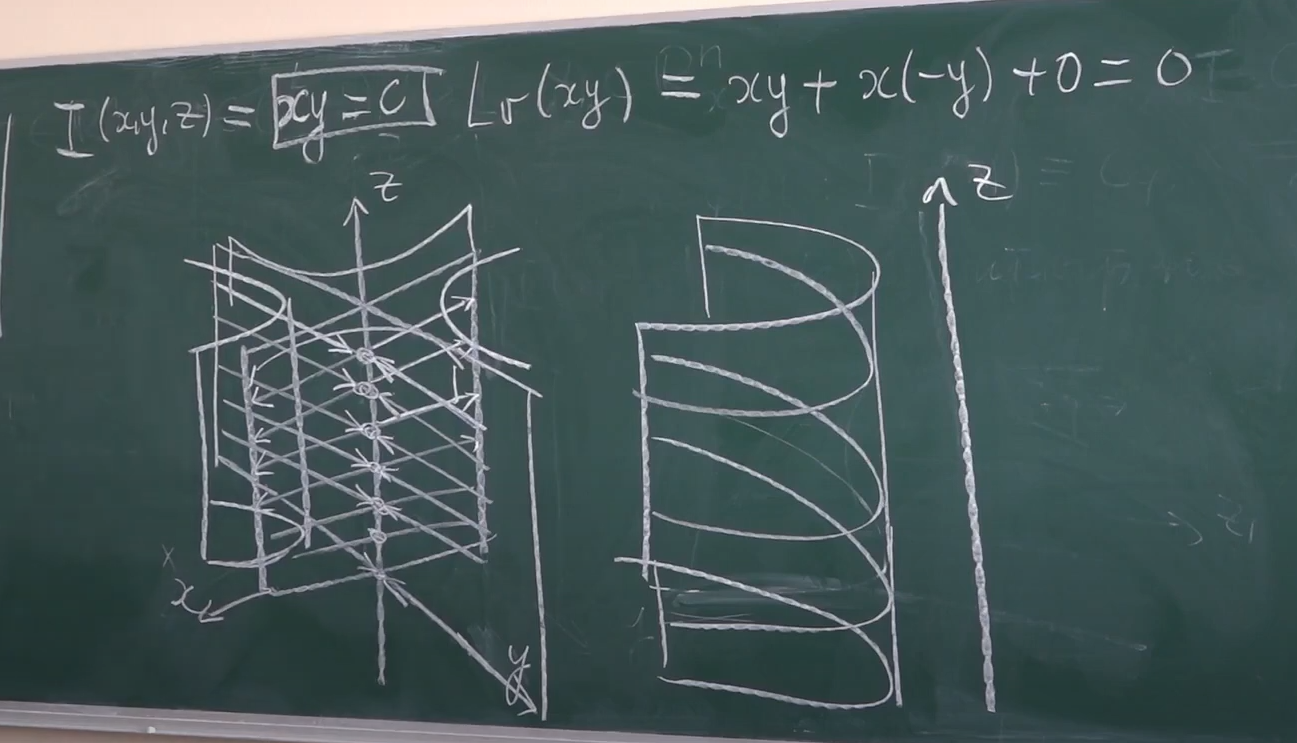
\includegraphics[scale=0.7]{img/hyper_rusalli.png}
	\end{figure}

\end{example}

\newpage
\begin{example}
	\[
		\begin{cases}
			\dot{x} = y  \\
			\dot{y} = -x \\
			\dot{z} = x^2 + y^2
		\end{cases}
	\]
	Одним из первых интегралов этой системы будет $I(x,\,y,\,z) = x^2 + y^2 = c \geq 0$. Аналогично, исслледуем фазовый портрет, используя этот ПИ.
	\begin{figure}[h]
		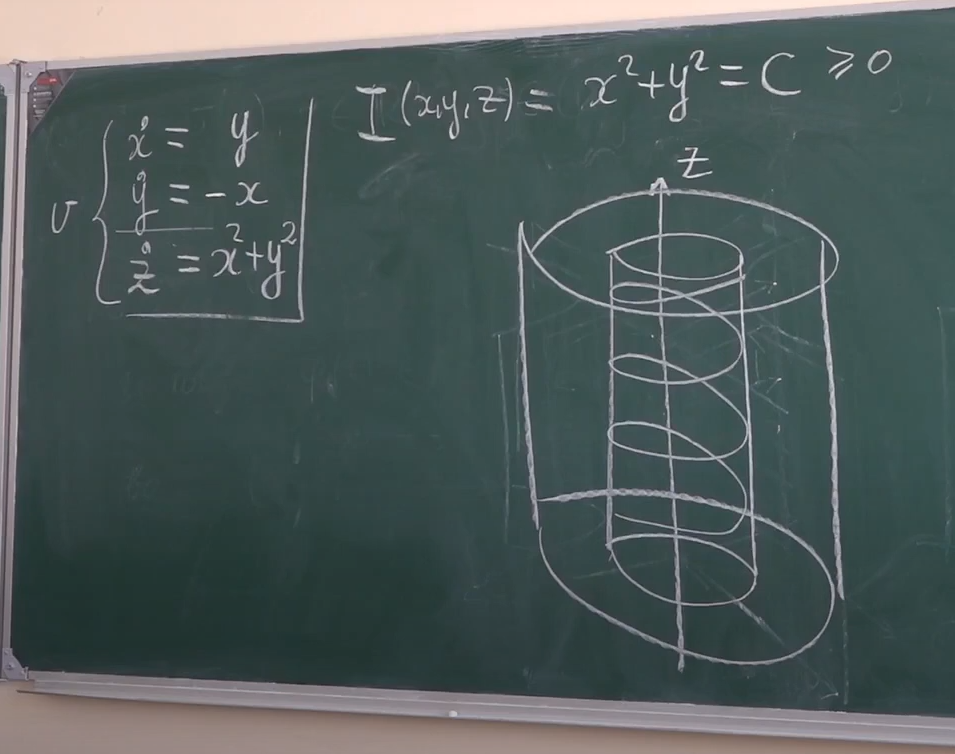
\includegraphics[scale=0.7]{img/paral_rusalli.png}
	\end{figure}
\end{example}

\newpage
\begin{example}
	Математический маятник.

	Используя закон сохранения энергии, получим один из первых интегралов системы, соответствующей движению математического маятника:
	\[\frac{m(l\dot{x})^2}{2} + mgl(1 - \cos x) = const\]
	Поделим на $ml^2$, продифференцируем по $t$ и получим уравнение математического маятника:
	\[\ddot{x} + \omega^2\sin x = 0\]
	При достаточно малых колебаниях $x$, можно использовать линеаризованное уравнение:
	\[\ddot{x} + \omega^2x = 0\]
	Это уравнение называется гармонический осцилятор, которое также является уравнением, соответствующим закону Гука и ещё много чему.
	Это уравнение сводится к системе:
	\[
		\begin{cases}
			\dot{y} = -\omega^2x \\
			\dot{x} = y
		\end{cases}
	\]
	Первым интегралом для линеаризованной системы является $I(x,\,y) = y^2 + \omega^2x^2 = const$. Для нелинеаризованного же маятника первым интегралом будет $I(x,\,y) = y^2 - \omega^2\cos x = const$. 

	С помощью этого первого интеграла мы теперь можем построить фазовый портрет математического маятника.
	\begin{figure}[h]
		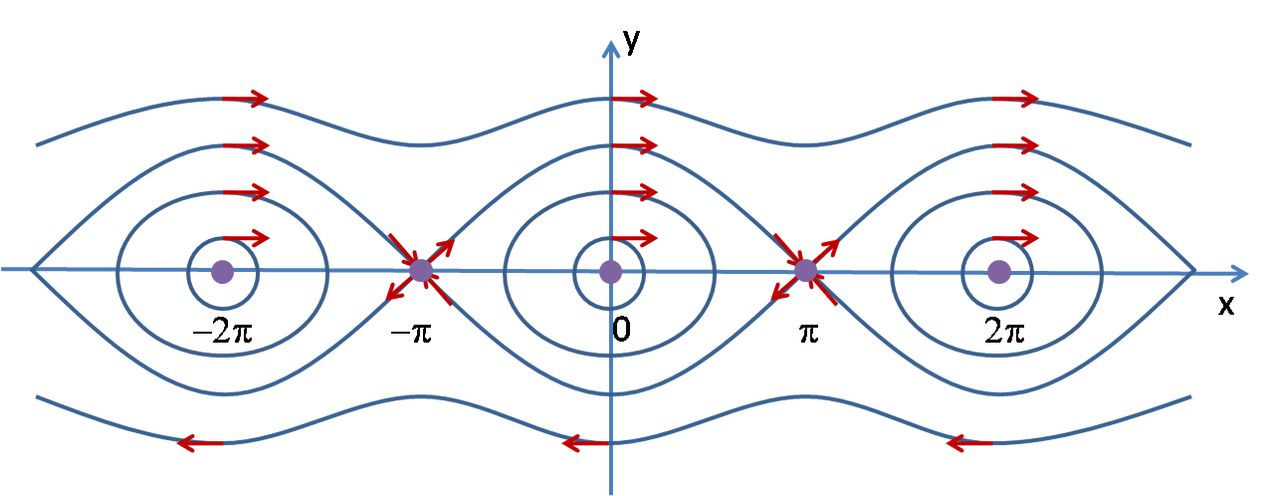
\includegraphics[scale = 0.7]{img/oscilator.png}
	\end{figure}
\end{example}

\subsection{Общее решение линейного однородного уравнения в частных производных первого порядка. Постановка задачи Коши. Теорема существования и единственности решения задачи Коши.}
\begin{definition}
	Уравнение вида
	\[F\left(x_1,\,\cdots,\,x_n,\, u,\, \frac{\partial u}{\partial x_1},\,\cdots,\,\frac{\partial u}{\partial x_n}\right) = 0\]
	где $n \geq 2,\, F(x_1,\,\cdots,\,x_n,\,u,\,p_1,\,\cdots,\,p_n)$ -- заданная действительная непрерывно дифференцируемая функция в некоторой области $G \subseteq \mathbb{R}^{2n + 1}$ и в каждой точке $G$:
	\[\sum_{i = 1}^n \left(\frac{\partial F}{\partial p_i}\right)^2 \neq 0\]
	называется дифференциальным уравнением в частных производных первого порядка относительно неизвестной функции $u = u(x_1,\,\cdots,\,x_n)$.
\end{definition}

\begin{definition}
	Функция $\phi(x_1,\,\cdots,\,x_n)$, заданная  в области $\Omega \subseteq \mathbb{R}^n_{(x_1,\,\cdots,\,x_n)}$ называется решением уравнения в частных производных, если:
	\begin{enumerate}
		\item $\phi(x_1,\,\cdots,\,x_n)$ -- непрерывно дифференцируемая функция в $\Omega$.
		\item Для всех точек $(x_1,\,\cdots,\,x_n) \in \Omega$ точка $(x_1,\,\cdots,\,x_n,\, \phi(x_1,\,\cdots,\,x_n),\, \frac{\partial \phi}{\partial x_1},\,\cdots,\,\frac{\partial \phi}{\partial x_n}) \in G$.
		\item $F(x_1,\,\cdots,\,x_n,\, \phi(x_1,\,\cdots,\,x_n),\, \frac{\partial \phi}{\partial x_1},\,\cdots,\,\frac{\partial \phi}{\partial x_n}) \equiv 0,\, \forall (x_1,\,\cdots,\,x_n) \in \Omega$.
	\end{enumerate}
\end{definition}

\begin{definition}
	Решение уравнения в частных производных в $(n + 1)$-мерном пространстве задаёт некоторую гладкую поверхность размерности $n$ (гиперповерхность), которая называется интегральной поверхностью этого уравнения.
\end{definition}

\begin{note}
	Если ввести вектор-функцию $a(x)$ с компонентами $a_1(x),\,\cdots,\,a_n(x)$, то уравнение в частных производных сокращённо можно записать с помощью скалярного произведения в следующем виде:
	\[(a(x),\, \text{grad }u(x)) = 0\]
\end{note}

\begin{definition}
	Автономная система
	\[\dot{x}(t) = a(x)\]
	называется характеристической системой уравнения в частных производных, а траектории системы называются характеристиками исходного уравнения.
\end{definition}

\begin{definition}
	Уравнение вида 
	\[\sum_{i = 1}^na_i(x_1,\,\cdots,\,x_n)\frac{\partial u}{\partial x_i} = 0\]
	называется линейным однородным уравнением в частных производных первого порядка.
\end{definition}

\begin{note}
	Пусть $x = (x_1,\,\cdots,\,x_n) \in \Omega \subseteq \mathbb{R}^n_x,\, n \geq 2$. В области $\Omega$ рассмотрим линейное однородное уравнение в частных производных первого порядка
	\[\sum_{i = 1}^n a_i(x)\frac{\partial u}{\partial x_i}(x) = 0\]
	где $a_i(x)$ -- заданные непрерывно дифференцируемые в $\Omega$ функции, для которых
	\[\sum_{i = 1}^n a_i^2(x) \neq 0, \forall x \in \Omega\]
	Это условие значит, что область $\Omega$ не содержит положений равновесия характеристической системы уравнения.
\end{note}

\begin{theorem}
	В некоторой окрестности каждой точки $b \in \Omega$ все решения уравнения имеют вид
	\[u(x) = F[u_1(x),\,\cdots,\,u_{n-1}(x)]\]
	где $u_j(x),\, j = \overline{1,\,n-1}$ -- независимые в точке $b$ первые интегралы характеристической системы, а $F(\zeta_1,\,\cdots,\,\zeta_n)$ -- произвольная непрерывно дифференцируемая функция.
\end{theorem}

\begin{proof}
	По критерию первого интеграла все решения уравнения в частных производных являются первыми интегралами характеристической системы, так как исходное уравнение равносильно тому, что производная в силу системы равна нулю в области $\Omega$.

	По теореме о количестве первых интегралов, в некоторой окрестности $V \subseteq \Omega$ точки $b \in \Omega$ существуют $(n-1)$ независимых в точке $b$ первых интегралов $u_1(x),\,\cdots,\,u_{n - 1}(x)$ характеристической системы и любой первый интеграл имеет вид, требуемый в условии этой теоремы.
\end{proof}

\begin{definition}
	Функция $u(x) = F[u_1(x),\,\cdots,\,u_{n-1}(x)]$, где $F$ -- произвольная непрерывно дифференцируемая функция своих аргументов, называется общим решением уравнения в частных производных в окрестности $V$ точки $b \in \Omega$.
\end{definition}

\begin{note}
	Из доказанной теоремы следует, что характеристики являются линиями уровня интегральной поверхности уравнения в частных производных.

	Пусть уравнение $g(x) = 0$ задаёт в области $\Omega$ гладкую $(n - 1)$-мерную поверхность $\gamma$. Эта поверхность называется начальной поверхностью, пусть, кроме того, на поверхности $\gamma$ задана некоторая непрерывно дифференцируемая функция $\phi(x)$.

	Зададим начальное условие
	\[u(x)|_{x \in \gamma} = \phi(x)\]
	Функция $\phi(x)$ называется начальным значением $u(x)$.

	\textbf{Задача Коши} для уравнения в частных производных: найти такое решение уравнения, которое удовлетворяет начальному условию.
\end{note}

\newpage
\subsubsection*{Геометрический смысл}
\begin{figure}[h]
	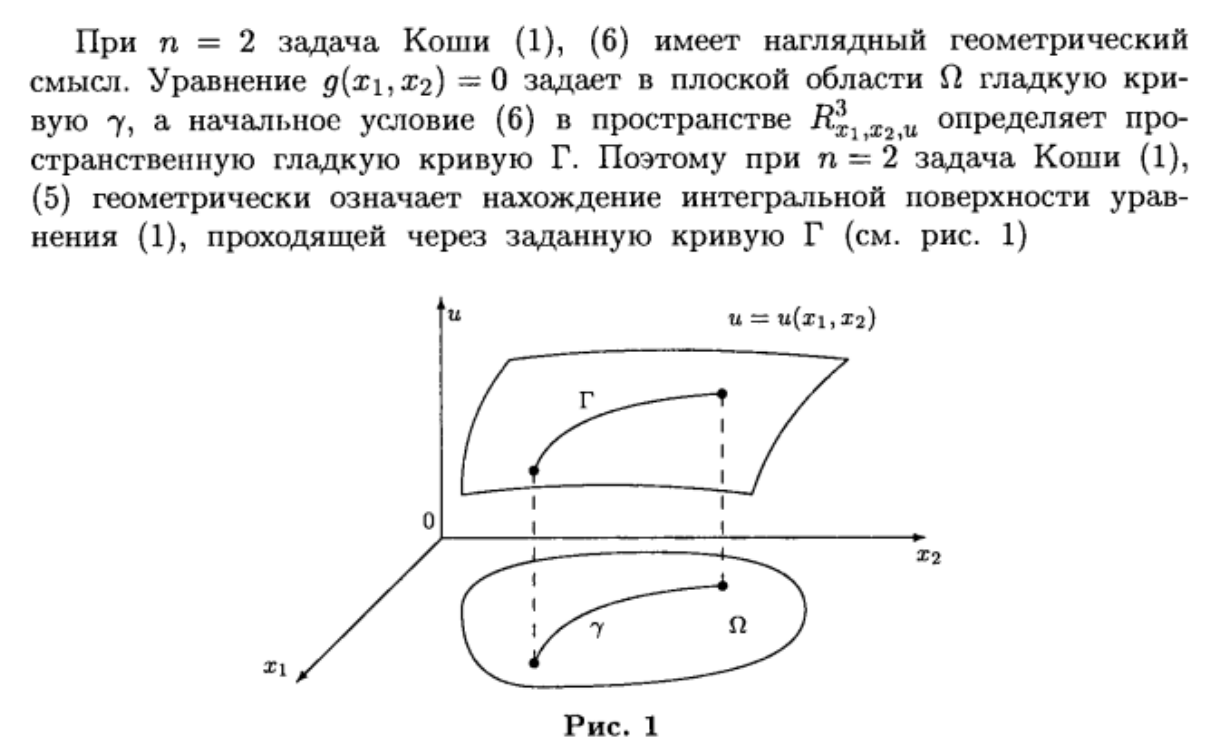
\includegraphics[scale=0.7]{img/geom_mean.png}
\end{figure}

\begin{definition}
	Всякая точка $M_0 \in \gamma$, для которой
	\[\overset{'}{g}(M_0) = (a(M_0),\,\text{grad }g(M_0)) = 0\]
	называется характеристической точкой уравнения в частных производных.
\end{definition}

\begin{note}
	Тот факт, что $M_0 \in \gamma$ является характеристической точкой уравнения, геометрически означает, что вектор $a(M_0)$ касается поверхности $\gamma$ в точке $M_0$ или, что то же самое, касается характеристик в точке $M_0$. В частности, положения равновесия характеристической системы и особые точки поверхности $\gamma$ являются характеристическими точками уравнения. Если при $n = 2$ кривая $\gamma$ является характеристикой уравнения, то каждая точка $\gamma$ является характеристической точкой.
\end{note}

\begin{theorem}
	Если $M_0 \in \gamma$ не является характеристической точкой уравнения, то в некоторой окрестности $V \subseteq \Omega$ точки $M_0$ решение задачи Коши в частных производных существует и единственно.
\end{theorem}

\begin{proof}
	Так как $M_0$ не характеристическая точка, то $a(M_0) \neq 0$, значит в некоторой окрестности $V$ точки $M_0$ существуют $(n-1)$ независимых в точке $M_0$ первых интегралов $u_i(x),\, i =\overline{1,\,n-1}$, характеристической системы. По теореме в окрестности $V$ общее решение имеет вид
	\[u(x) = F[u_1(x),\,\cdots,\,u_{n - 1}(x)]\]
	где $F$ -- непрерывно дифференцируемая функция. 
	
	Покажем, что начальное условие однозначно определяет вид функции $F$. С этой целью в окрестности $V$ рассмотрим систему уравнений
	\[\begin{cases}
		u_i(x) = u_i,\, i = \overline{1,\,n-1}\\
		g(x) = 0
	\end{cases}\]
	Покажем, что эту систему можно однозначно разрешить относительно $x$ в окрестности $V$. Проверим для системы выполнение условий теоремы о системе неявных функций.

	Все функции в системе непрерывно дифференцируемы в окрестности $V$. Осталось показать, что якобиан
	\[\frac{\partial(u_1,\,\cdots,\,u_{n-1},\,g)}{\partial(x_1,\,\cdots,\,x_n)} \neq 0\]
	Рассуждаем от противного, пусть якобиан равен нулю. Так как первые $(n-1)$ строк якобиана линейно независимы, то в таком случае последняя его строка линейно зависит от его первых $(n-1)$ строк. Следовательно, найдутся числа $c_i,\, i = \overline{1,\,n-1}$, одновременно не равные нулю, такие, что
	\[\frac{\partial g(M_0)}{\partial x_j} = \sum_{i = 1}^{n-1}c_i\frac{\partial u_i(M_0)}{\partial x_j},\, \forall j = \overline{1,\,n}\]
	Поэтому
	\begin{align*}
		\overset{`}{g}(M_0) = \sum_{j = 1}^n a_j(M_0)\frac{\partial g(M_0)}{\partial x_j} = \sum_{j = 1}^n a_j(M_0)\sum_{i = 1}^{n-1}c_i\frac{\partial u_i(M_0)}{\partial x_j} = \\
		\sum_{i = n-1}^n c_i \sum_{j = 1}^{n-1} a_j(M_0)\frac{\partial u_i(M_0)}{\partial x_j} = \sum_{i = 1}^{n-1}c_i\overset{`}{u}_i(M_0) = 0
	\end{align*}
	С другой стороны, $\overset{`}{g}(M_0) \neq 0$, так как по условию теоремы $M_0 \in \gamma$ не является характеристической точкой уравнения. Противоречие.

	Поэтому в окрестности $V$ выполнены все условия теоремы о неявной функции и система уравнений допускает в окрестности $V$ единственное непрерывно дифференцируемое решение $x = \omega(u_1,\,\cdots,\,u_{n-1})$.

	Для всех $x \in \gamma \cap V$ функция
	\[\phi(x) = \phi[\omega(u_1,\,\cdots,\,u_{n-1}]= \Phi(u_1,\,\cdots,\,u_{n-1})\]
	является известной непрерывно дифференцируемой функцией. По построению отсюда следует, что
	\[u(x) = \Phi[u_1(x),\,\cdots,\,u_{n-1}(x)]\]
	является искомым и единственным решением задачи Коши в окрестности $V$.
\end{proof}

\end{document}